\begin{appendices}
\chapter{Publications \label{chap:publications}}
% \section{Paper 1}
\clearpage
\addcontentsline{toc}{section}{Paper 1}
\includearticle[numbers=low]{pdf/SPE.pdf}
% \section{Paper 2}
\clearpage
\addcontentsline{toc}{section}{Paper 2}
\includearticle[numbers=low]{pdf/ICOUR.pdf}
% \section{Paper 3}
\clearpage
\addcontentsline{toc}{section}{Paper 3}
\includearticle[numbers=low]{pdf/energies-mdpi.pdf}

\chapter{Overview of tested gel systems \label{chap:gelSystem}}

\section{Table of gel systems}
\textbf{T}: Temperature\\
\textbf{$C_{\text{x}}$}: Concentration of x

\begin{center}
\begin{longtable}{|c|c|c|c|c|c|c|c|c|}
\caption{Overview of all prepared and tested gel systems}\\
\hline
\textbf{Series} & \textbf{T} &  \textbf{Polymer} & \textbf{$C_{\text{Pol}}$} & \textbf{\textbf{$C_{\text{\ce{Cr^3+}}}$}} & \textbf{$C_{\text{NP}}$} & \textbf{$C_{\text{PVS}}$} &
\multirow{2}{2em}{\textbf{$\frac{C_{\text{Pol}}}{C_{\text{NP}}}$}} &
\multirow{2}{2em}{\textbf{$\frac{C_{\text{NP}}}{C_{\text{PVS}}}$}} \\
 & [\celsius] & & [wt\%] & [ppm] & [wt\%] & [wt\%] & & \\
\hline
\endfirsthead
\multicolumn{9}{c}%
{\tablename\ \thetable\ -- \textit{Continued from previous page}} \vspace{.7cm}\\
\hline
\textbf{Series} & \textbf{T} &  \textbf{Polymer} & \textbf{$C_{\text{Pol}}$} & \textbf{\textbf{$C_{\text{\ce{Cr^3+}}}$}} & \textbf{$C_{\text{NP}}$} & \textbf{$C_{\text{PVS}}$} &
\multirow{2}{2em}{\textbf{$\frac{C_{\text{Pol}}}{C_{\text{NP}}}$}} &
\multirow{2}{2em}{\textbf{$\frac{C_{\text{NP}}}{C_{\text{PVS}}}$}} \\
 & [\celsius] & & [wt\%] & [ppm] & [wt\%] & [wt\%] & & \\
\hline
\endhead
\hline \multicolumn{9}{r}{\textit{Continued on next page}} \\
\endfoot
\hline
\endlastfoot
1	&	50	&	Flopaam 	&	0.994	&	101	&		&		&		&		\\
2	&	50	&	Alcoflood	&	1.000	&	101	&		&		&		&		\\
3	&	50	&	Alcomer	&	0.999	&	104	&		&		&		&		\\
4	&	50	&	Alcoflood	&	1.005	&		&	1.111	&		&	0.90	&		\\
5	&	50	&	Alcomer	&	0.998	&		&	1.098	&		&	0.91	&		\\
6	&	50	&	Flopaam 	&	0.496	&		&	1.087	&		&	0.46	&		\\
7	&	50	&	Alcoflood	&	1.003	&		&	1.062	&		&	0.94	&		\\
8	&	50	&	Alcomer	&	0.990	&		&	1.064	&		&	0.93	&		\\
9	&	50	&	Flopaam 	&	0.500	&		&	0.533	&		&	0.94	&		\\
10	&	50	&	Alcomer	&	0.499	&	129	&		&		&		&		\\
11	&	50	&	Alcomer	&	0.502	&	156	&		&		&		&		\\
12	&	50	&	Alcoflood	&	1.996	&	301	&		&		&		&		\\
13a,b,c	&	50	&	Alcoflood	&	0.502	&	107	&		&		&		&		\\
13d,e,f	&	50	&	Alcoflood	&	1.000	&	215	&		&		&		&		\\
13g,h,i	&	50	&	Alcoflood	&	1.994	&	419	&		&		&		&		\\
14a,b	&	50	&	Alcoflood	&	0.508	&	446	&		&		&		&		\\
14c,d	&	50	&	Alcoflood	&	1.003	&	409	&		&		&		&		\\
15	&	50	&	Flopaam 	&	0.500	&	99	&		&		&		&		\\
16	&	50	&	Alcomer	&	0.502	&	105	&		&		&		&		\\
17	&	80	&	Alcomer	&	1.002	&		&	0.380	&	0.053	&	2.64	&	7.16	\\
18	&	80	&	Alcomer	&	1.004	&		&	0.381	&	0.136	&	2.64	&	2.80	\\
19	&	80	&	Alcomer	&	0.931	&		&	0.352	&	0.273	&	2.64	&	1.29	\\
20	&	80	&	Alcomer	&	1.000	&		&	0.436	&		&	2.30	&		\\
21	&	80	&	Alcomer	&	1.001	&		&	0.646	&		&	1.55	&		\\
22	&	80	&	Alcomer	&	1.011	&		&	1.024	&		&	0.99	&		\\
23	&	80	&	Alcoflood	&	1.932	&		&	3.038	&		&	0.64	&		\\
24	&	80	&	Alcoflood	&	1.932	&		&	3.032	&		&	0.64	&		\\
25	&	80	&	Alcomer	&	0.249	&	22	&		&		&		&		\\
26	&	80	&	Alcomer	&	0.500	&	30	&		&		&		&		\\
27	&	80	&	Alcomer	&	0.999	&	30	&		&		&		&		\\
28	&	80	&	Alcomer	&	0.251	&	58	&		&		&		&		\\
29	&	80	&	Alcomer	&	0.500	&	53	&		&		&		&		\\
30	&	80	&	Alcomer	&	0.997	&	64	&		&		&		&		\\
31	&	80	&	Alcomer	&	0.248	&	109	&		&		&		&		\\
32	&	80	&	Alcomer	&	0.498	&	111	&		&		&		&		\\
33	&	80	&	Alcomer	&	0.995	&	113	&		&		&		&		\\
34	&	80	&	Alcoflood	&	1.932	&		&	3.039	&		&	0.64	&		\\
35	&	80	&	Alcomer	&	0.498	&	119	&		&		&		&		\\
36	&	80	&	Flopaam 	&	0.490	&	115	&		&		&		&		\\
37	&	80	&	Alcomer	&	1.000	&		&	0.380	&	0.054	&	2.63	&	7.05	\\
38	&	80	&	Flopaam 	&	1.003	&		&	0.381	&	0.054	&	2.63	&	7.06	\\
39	&	80	&	Alcoflood	&	1.999	&		&	0.381	&	0.054	&	5.24	&	7.12	\\
40	&	80	&	Alcomer	&	0.502	&		&	0.381	&	0.054	&	1.32	&	7.06	\\
41	&	80	&	Flopaam 	&	0.502	&		&	0.381	&	0.054	&	1.32	&	7.12	\\
42	&	80	&	Alcomer	&	0.500	&	60	&		&		&		&		\\
43	&	80	&	Alcomer	&	0.500	&	31	&		&		&		&		\\
44	&	80	&	Alcomer	&	0.997	&		&	0.191	&	0.027	&	5.23	&	7.05	\\
45	&	80	&	Alcomer	&	0.997	&		&	0.096	&	0.013	&	10.40	&	7.12	\\
46	&	80	&	Alcomer	&	0.505	&	41	&		&		&		&		\\
47	&	80	&	Alcoflood	&	1.931	&		&	3.036	&		&	0.64	&		\\
\end{longtable}
\label{tab:gelSystemSummary}
\end{center}


\section{Viscosity charts for gel systems}
What follows is a list of charts illustrating how the viscosity of the different prepared samples changed with time. 
\begin{figure}
    \makebox[\linewidth][c]{%
     \begin{subfigure}[b]{0.6\textwidth}
         \centering
         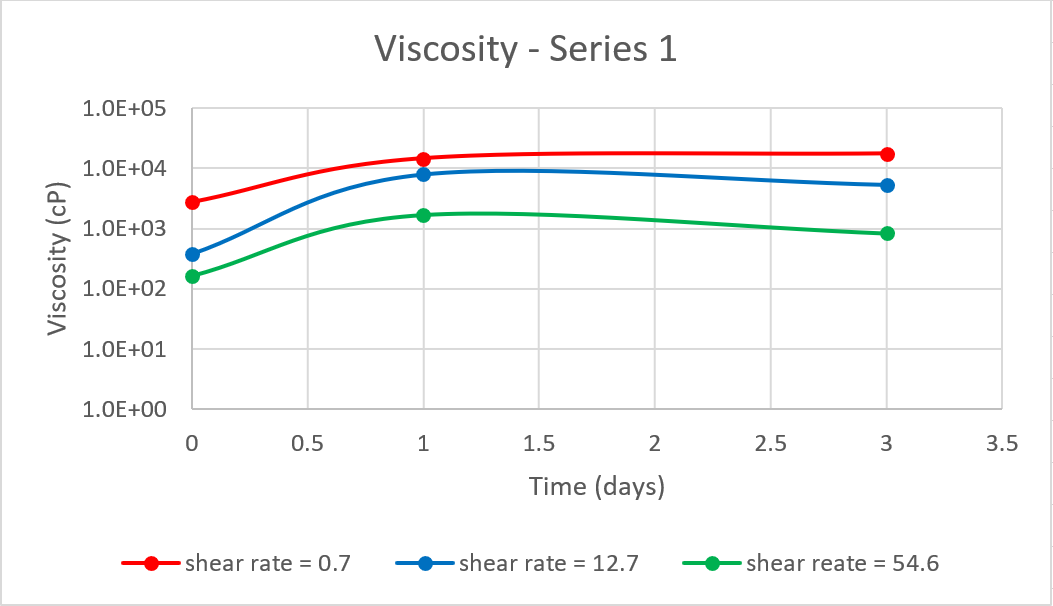
\includegraphics[width=\textwidth]{img/visc/1.png}
     \end{subfigure}
    %  \hfill
     \begin{subfigure}[b]{0.6\textwidth}
         \centering
         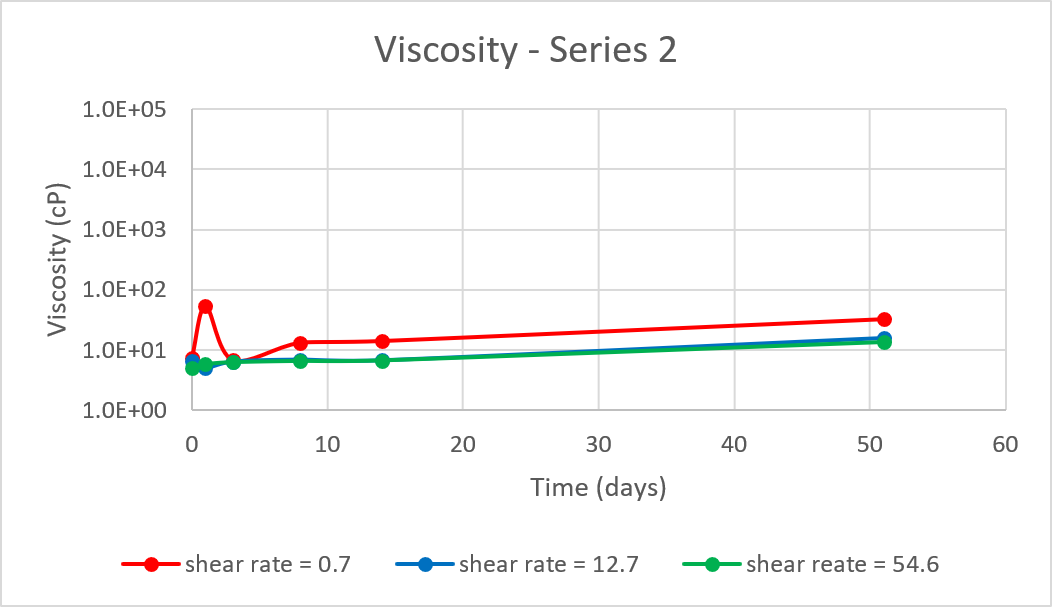
\includegraphics[width=\textwidth]{img/visc/2.png}
     \end{subfigure}
    }\\
    \makebox[\linewidth][c]{%
     \begin{subfigure}[b]{0.6\textwidth}
         \centering
         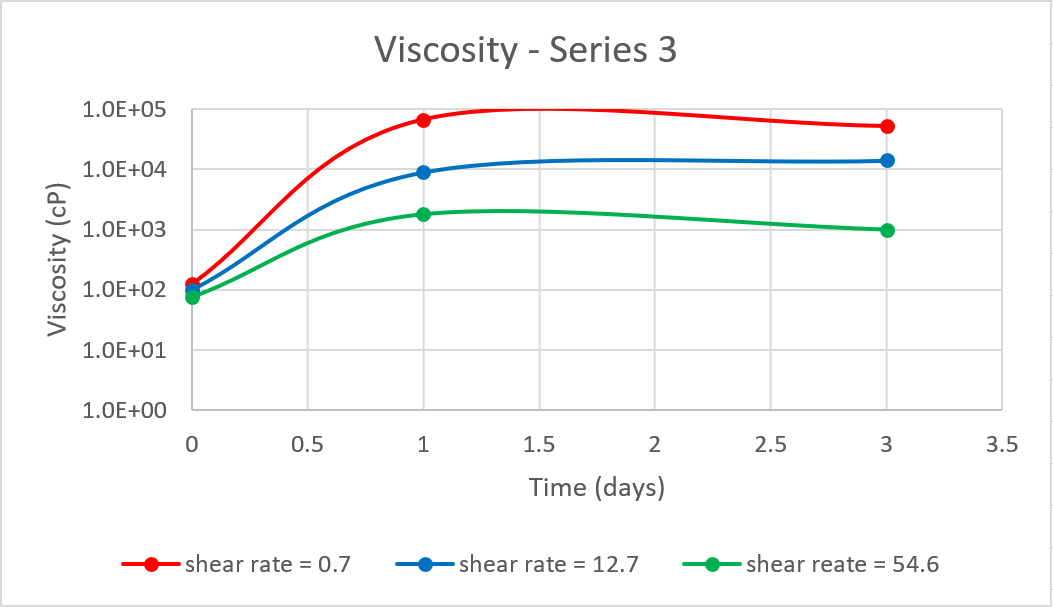
\includegraphics[width=\textwidth]{img/visc/3.png}
     \end{subfigure}
    %  \hfill
     \begin{subfigure}[b]{0.6\textwidth}
         \centering
         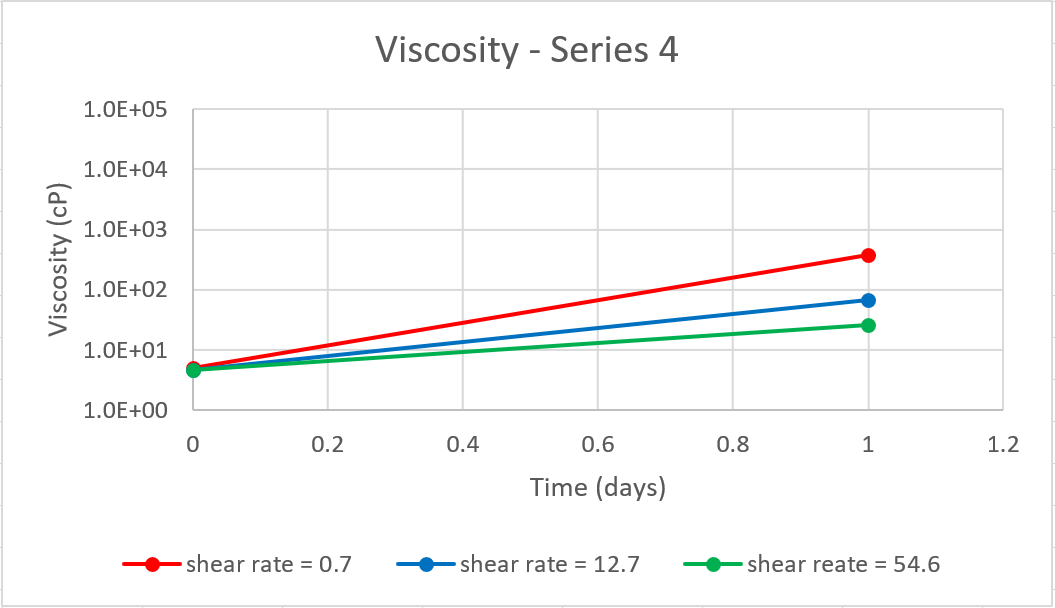
\includegraphics[width=\textwidth]{img/visc/4.png}
     \end{subfigure}
    }\\
    \makebox[\linewidth][c]{%
     \begin{subfigure}[b]{0.6\textwidth}
         \centering
         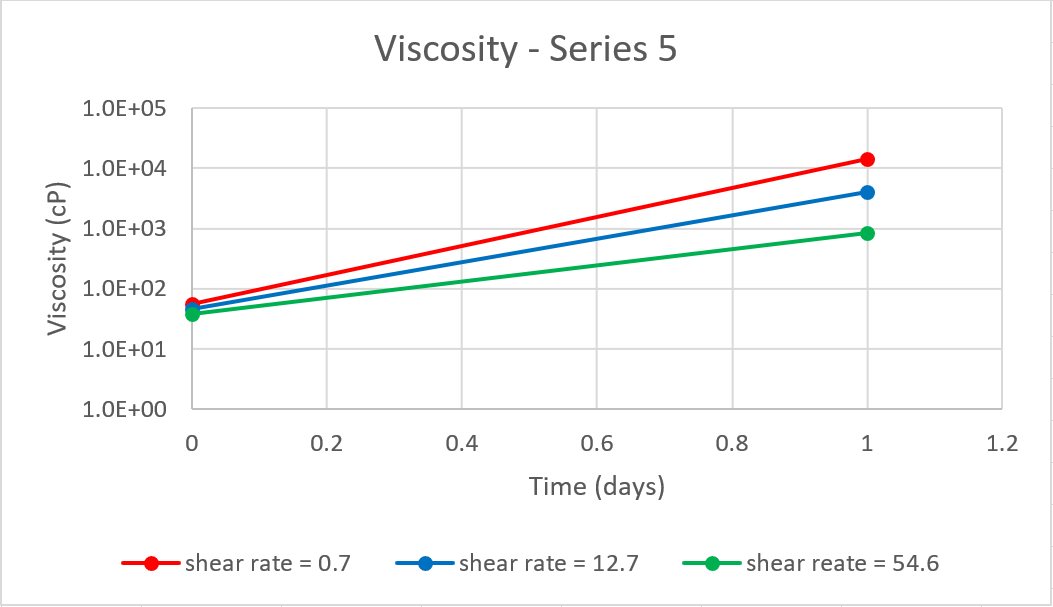
\includegraphics[width=\textwidth]{img/visc/5.png}
     \end{subfigure}
    %  \hfill
     \begin{subfigure}[b]{0.6\textwidth}
         \centering
         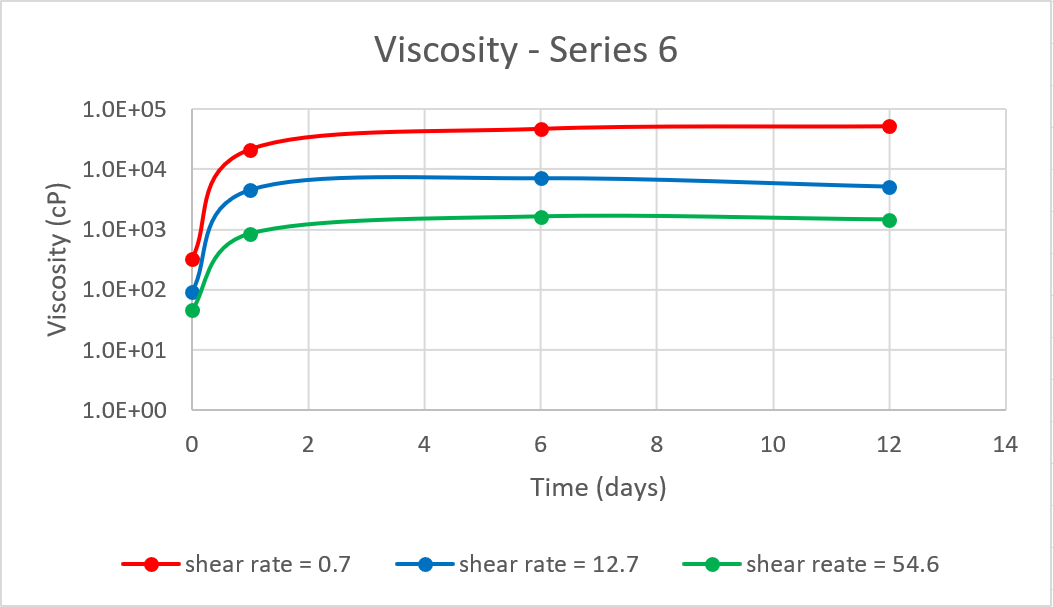
\includegraphics[width=\textwidth]{img/visc/6.png}
     \end{subfigure}
    }\\
    \makebox[\linewidth][c]{%
     \begin{subfigure}[b]{0.6\textwidth}
         \centering
         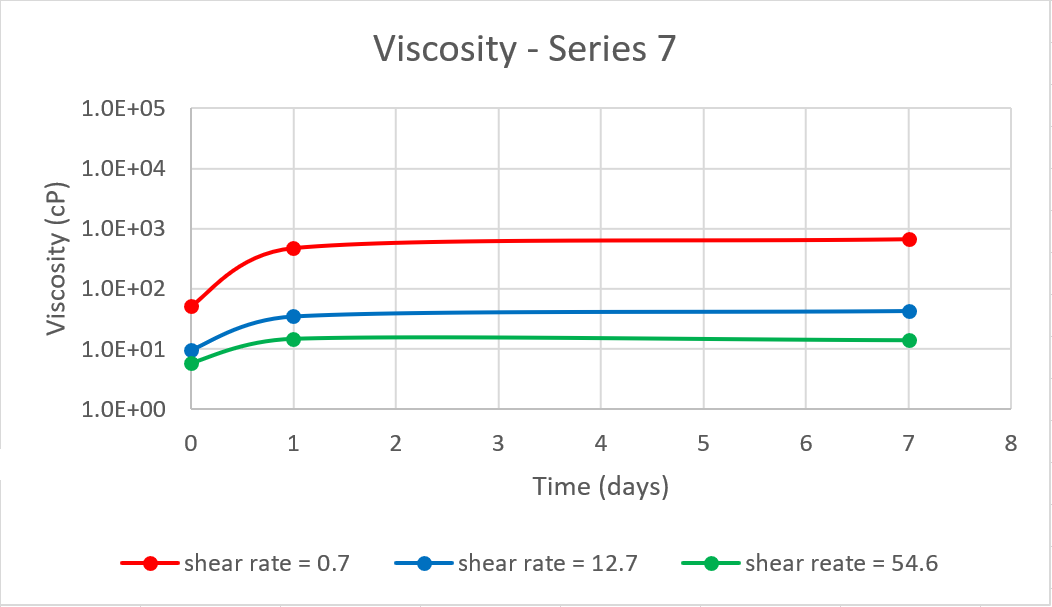
\includegraphics[width=\textwidth]{img/visc/7.png}
     \end{subfigure}
    %  \hfill
     \begin{subfigure}[b]{0.6\textwidth}
         \centering
         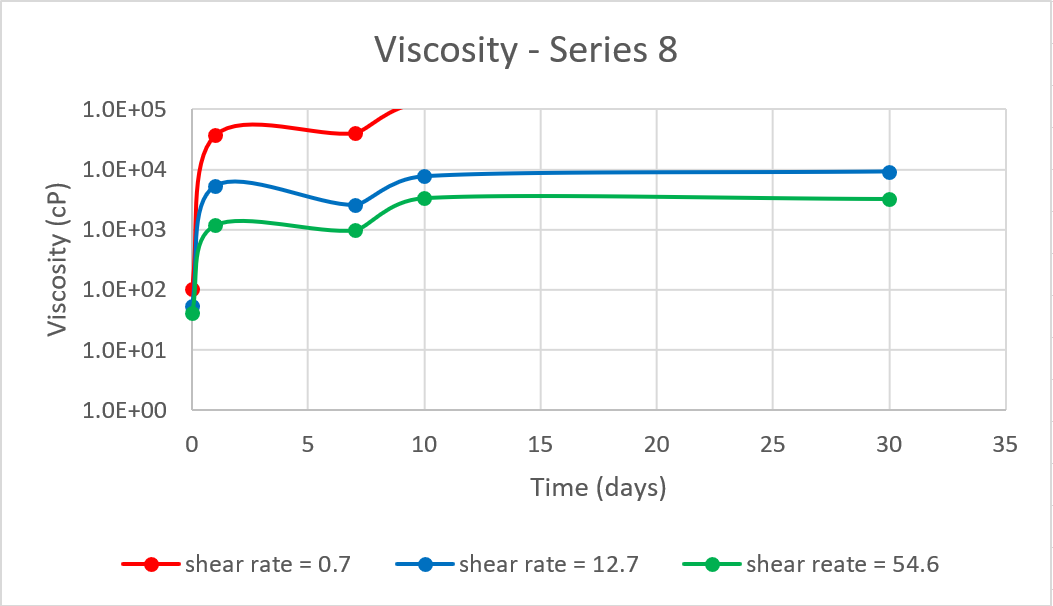
\includegraphics[width=\textwidth]{img/visc/8.png}
     \end{subfigure}
    }\\
        \caption{Viscosity vs. time, series 1 through 8}
        \label{fig:visc1-8}
\end{figure}


\begin{figure}
    \makebox[\linewidth][c]{%
     \begin{subfigure}[b]{0.6\textwidth}
         \centering
         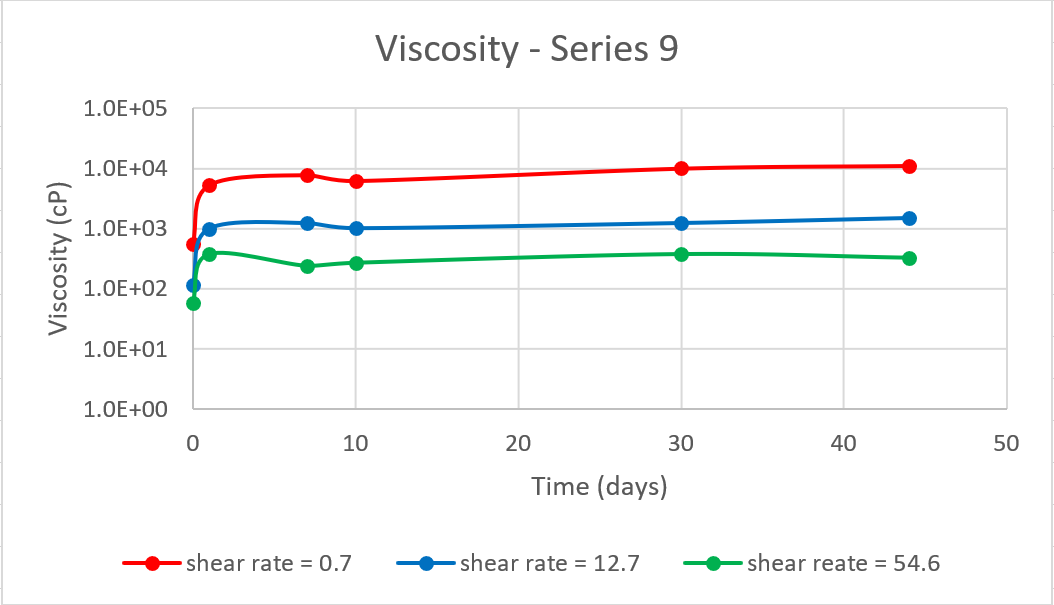
\includegraphics[width=\textwidth]{img/visc/9.png}
     \end{subfigure}
    %  \hfill
     \begin{subfigure}[b]{0.6\textwidth}
         \centering
         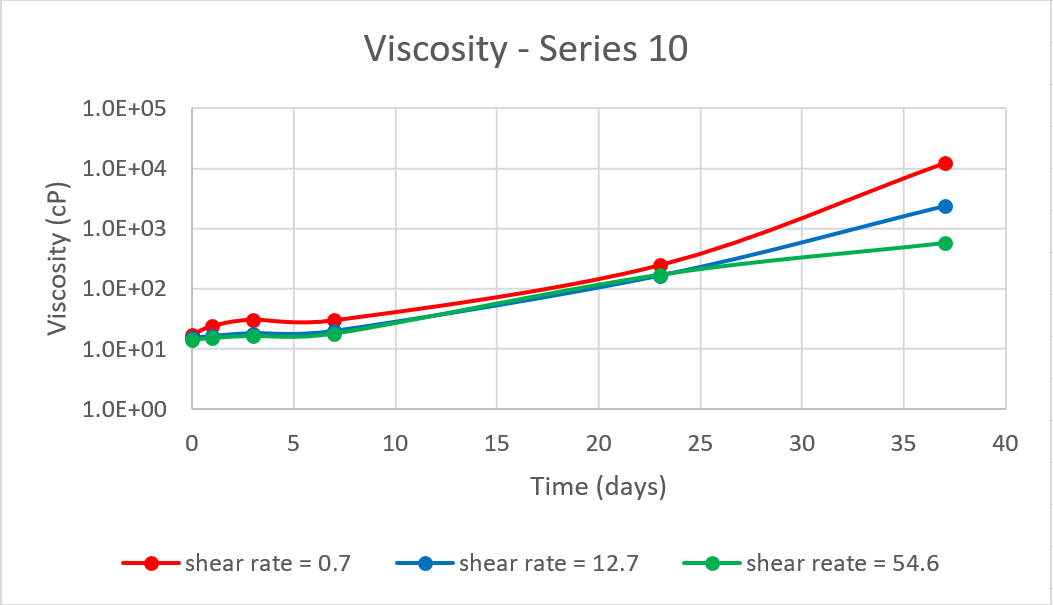
\includegraphics[width=\textwidth]{img/visc/10.png}
     \end{subfigure}
    }\\
    \makebox[\linewidth][c]{%
     \begin{subfigure}[b]{0.6\textwidth}
         \centering
         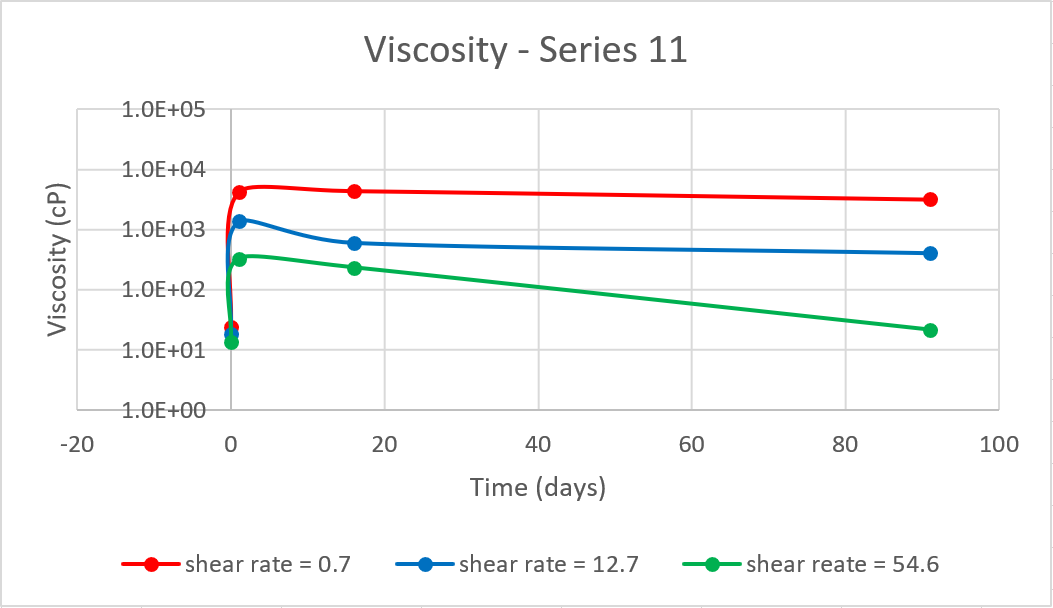
\includegraphics[width=\textwidth]{img/visc/11.png}
     \end{subfigure}
    %  \hfill
     \begin{subfigure}[b]{0.6\textwidth}
         \centering
         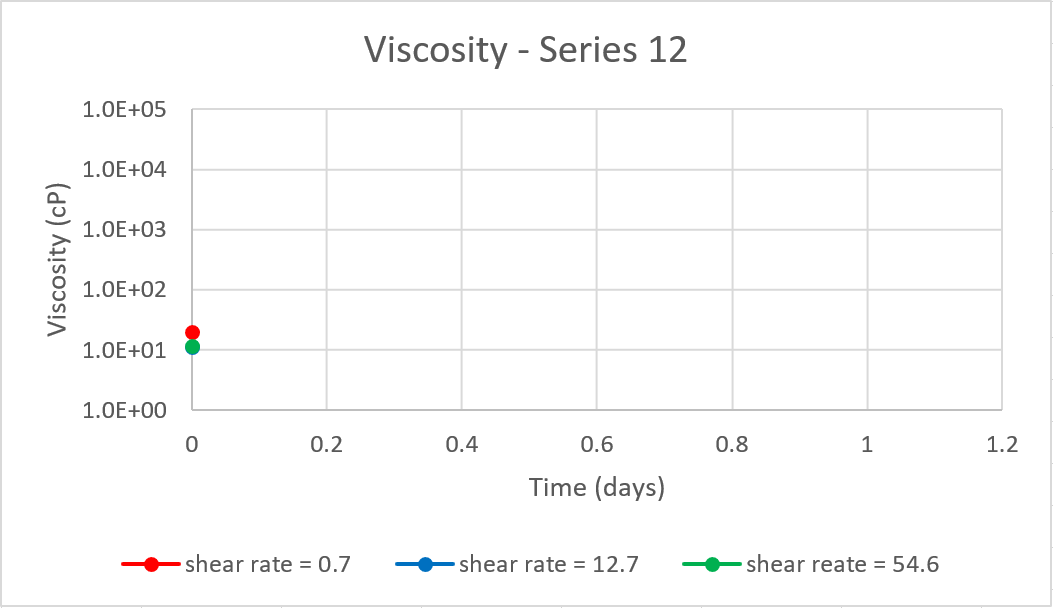
\includegraphics[width=\textwidth]{img/visc/12.png}
     \end{subfigure}
    }\\
    \makebox[\linewidth][c]{%
     \begin{subfigure}[b]{0.6\textwidth}
         \centering
         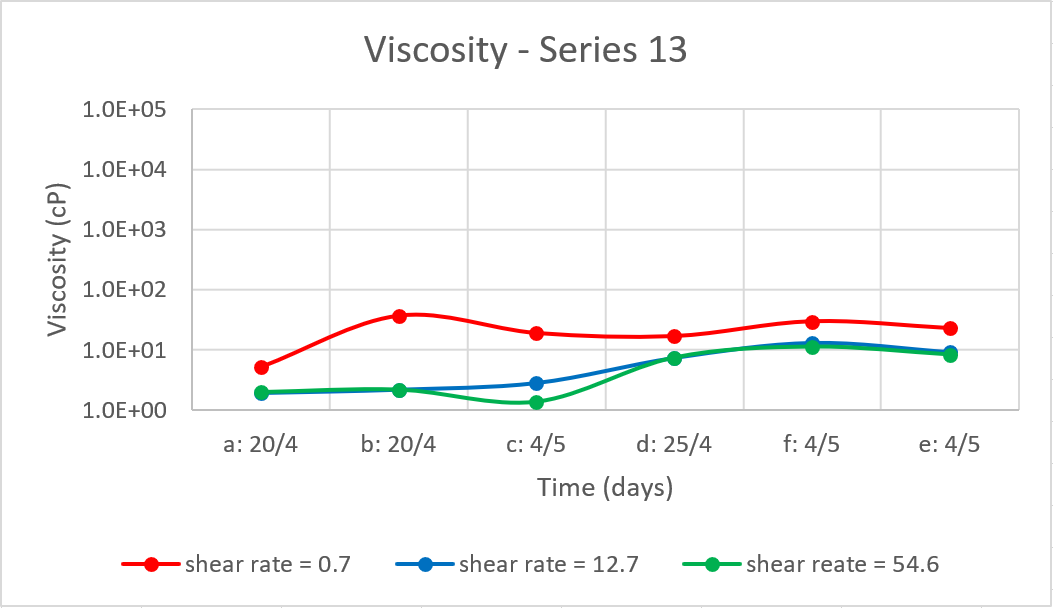
\includegraphics[width=\textwidth]{img/visc/13.png}
     \end{subfigure}
    %  \hfill
     \begin{subfigure}[b]{0.6\textwidth}
         \centering
         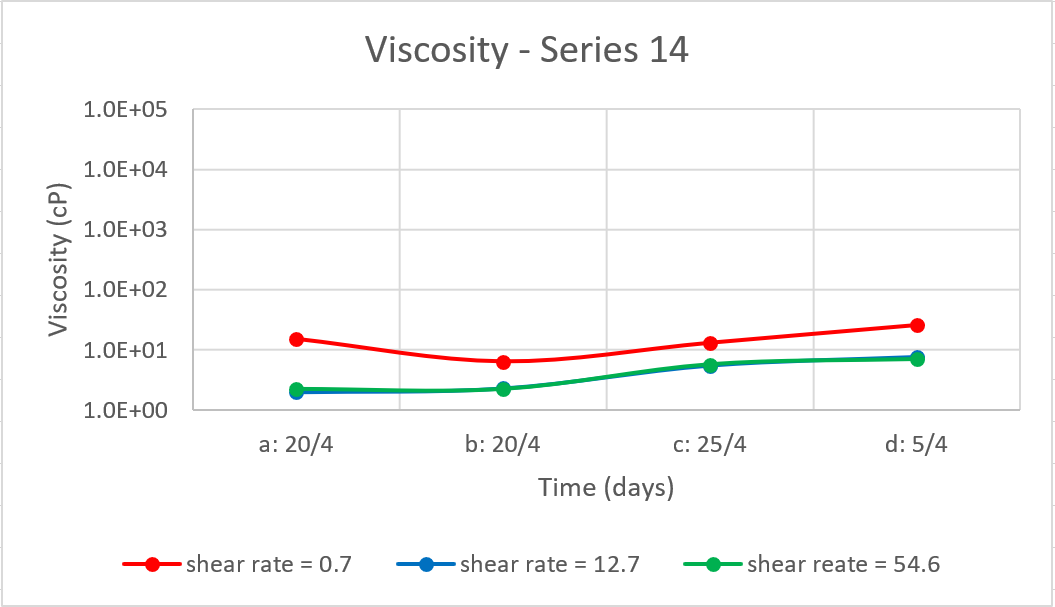
\includegraphics[width=\textwidth]{img/visc/14.png}
     \end{subfigure}
    }\\
    \makebox[\linewidth][c]{%
     \begin{subfigure}[b]{0.6\textwidth}
         \centering
         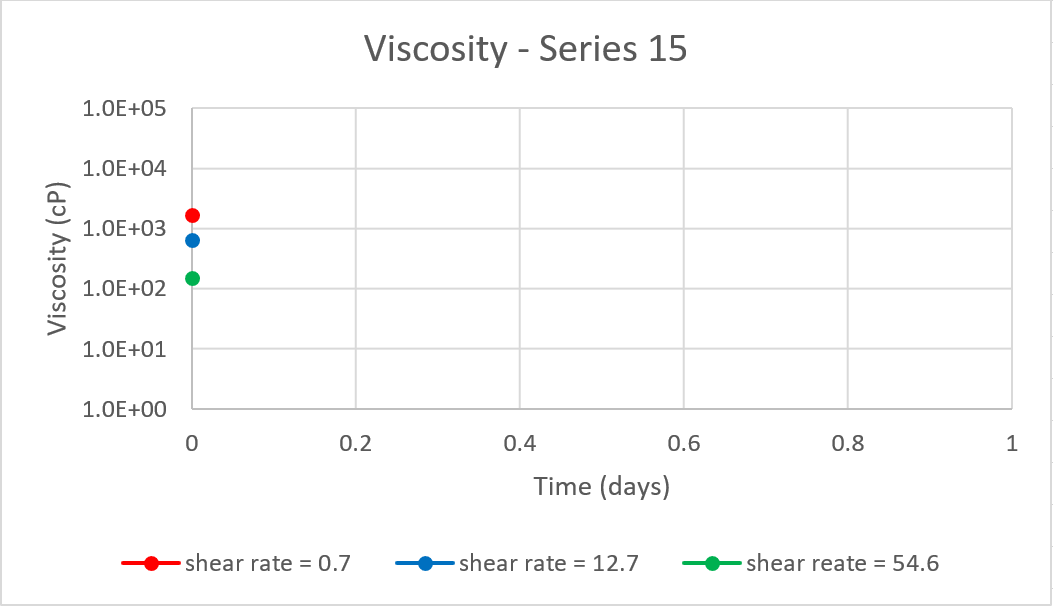
\includegraphics[width=\textwidth]{img/visc/15.png}
     \end{subfigure}
    %  \hfill
     \begin{subfigure}[b]{0.6\textwidth}
         \centering
         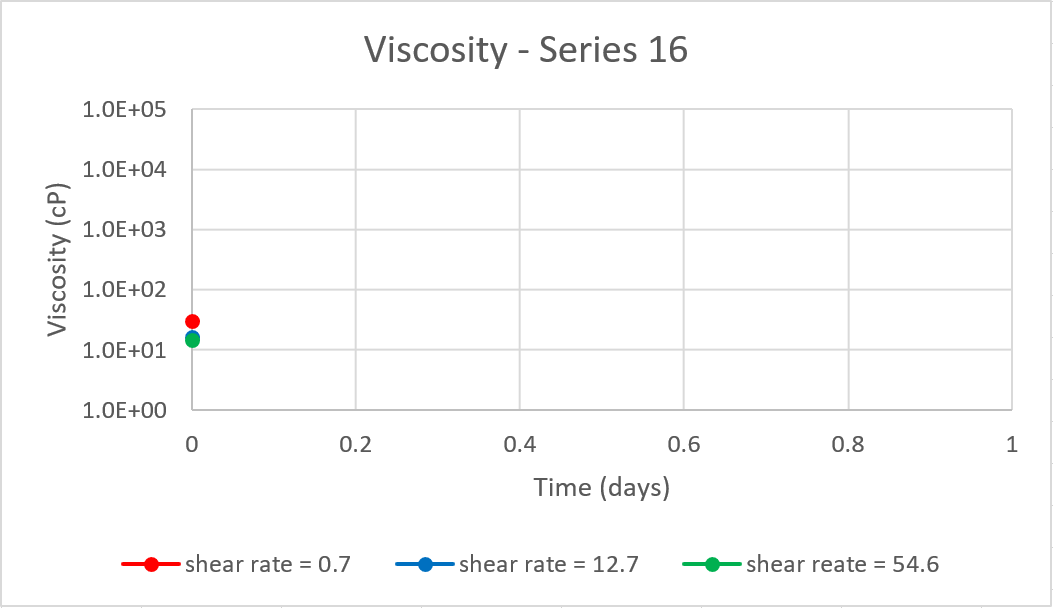
\includegraphics[width=\textwidth]{img/visc/16.png}
     \end{subfigure}
    }\\
        \caption{Viscosity vs. time, series 9 through 16}
        \label{fig:visc9-16}
\end{figure}


\begin{figure}
    \makebox[\linewidth][c]{%
     \begin{subfigure}[b]{0.6\textwidth}
         \centering
         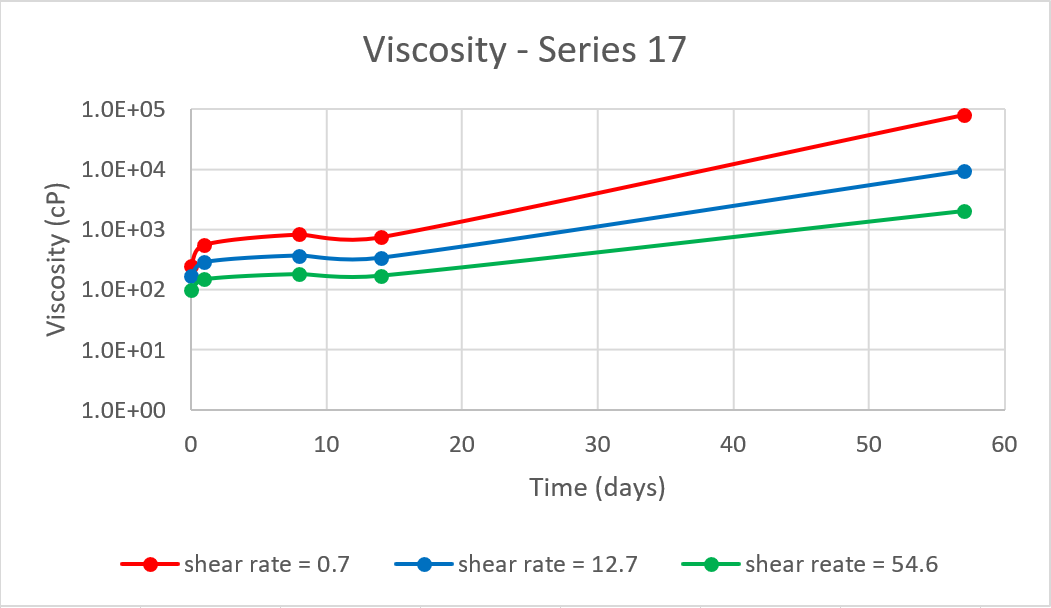
\includegraphics[width=\textwidth]{img/visc/17.png}
     \end{subfigure}
    %  \hfill
     \begin{subfigure}[b]{0.6\textwidth}
         \centering
         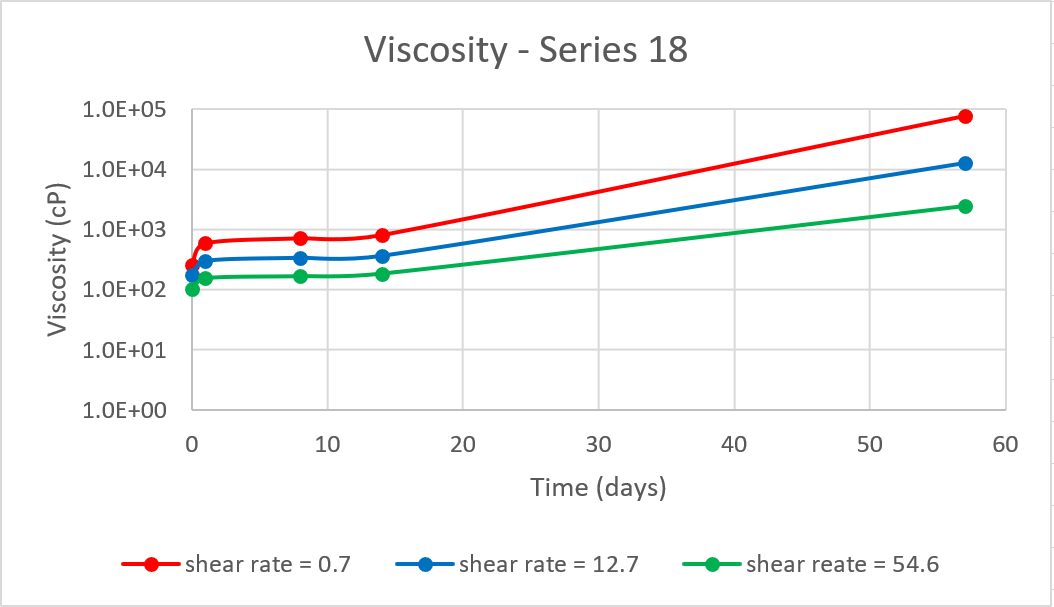
\includegraphics[width=\textwidth]{img/visc/18.png}
     \end{subfigure}
    }\\
    \makebox[\linewidth][c]{%
     \begin{subfigure}[b]{0.6\textwidth}
         \centering
         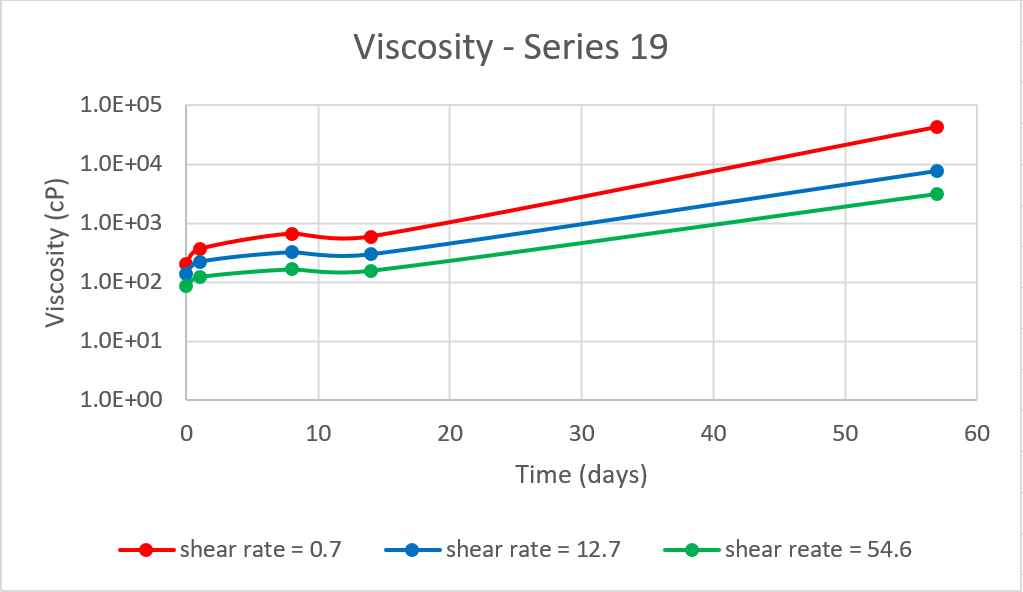
\includegraphics[width=\textwidth]{img/visc/19.png}
     \end{subfigure}
    %  \hfill
     \begin{subfigure}[b]{0.6\textwidth}
         \centering
         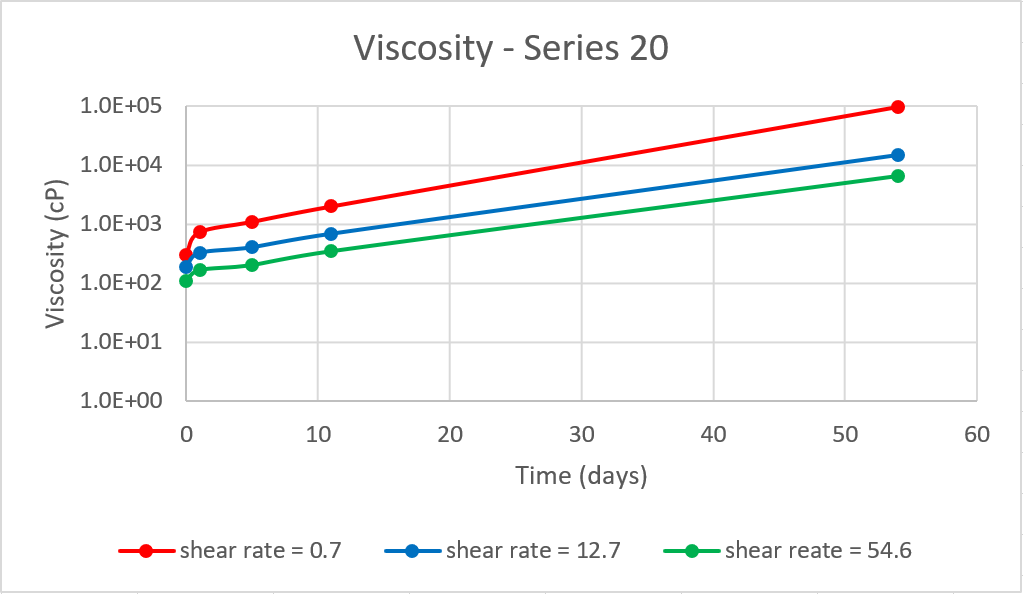
\includegraphics[width=\textwidth]{img/visc/20.png}
     \end{subfigure}
    }\\
    \makebox[\linewidth][c]{%
     \begin{subfigure}[b]{0.6\textwidth}
         \centering
         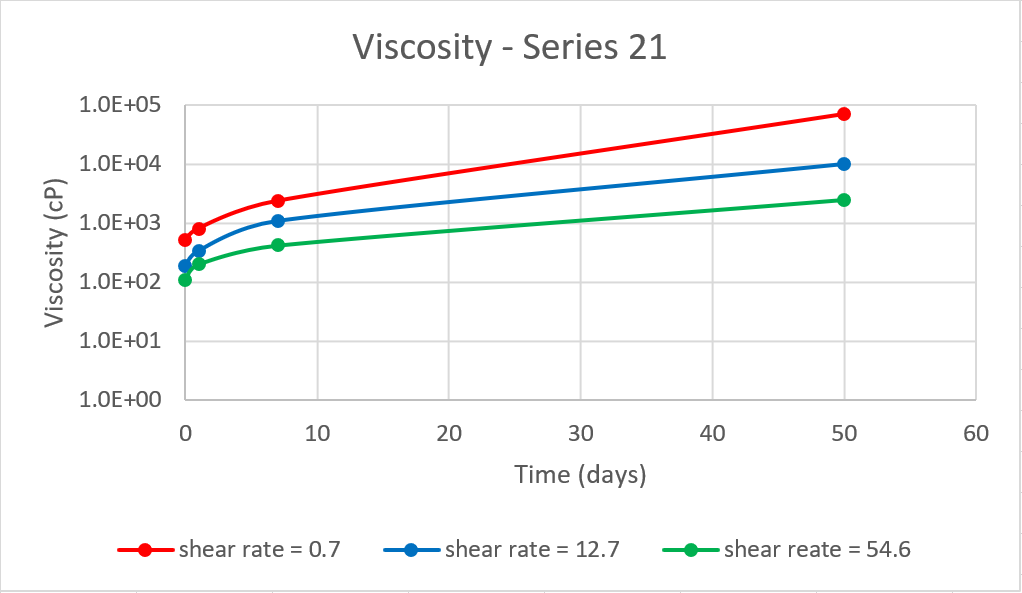
\includegraphics[width=\textwidth]{img/visc/21.png}
     \end{subfigure}
    %  \hfill
     \begin{subfigure}[b]{0.6\textwidth}
         \centering
         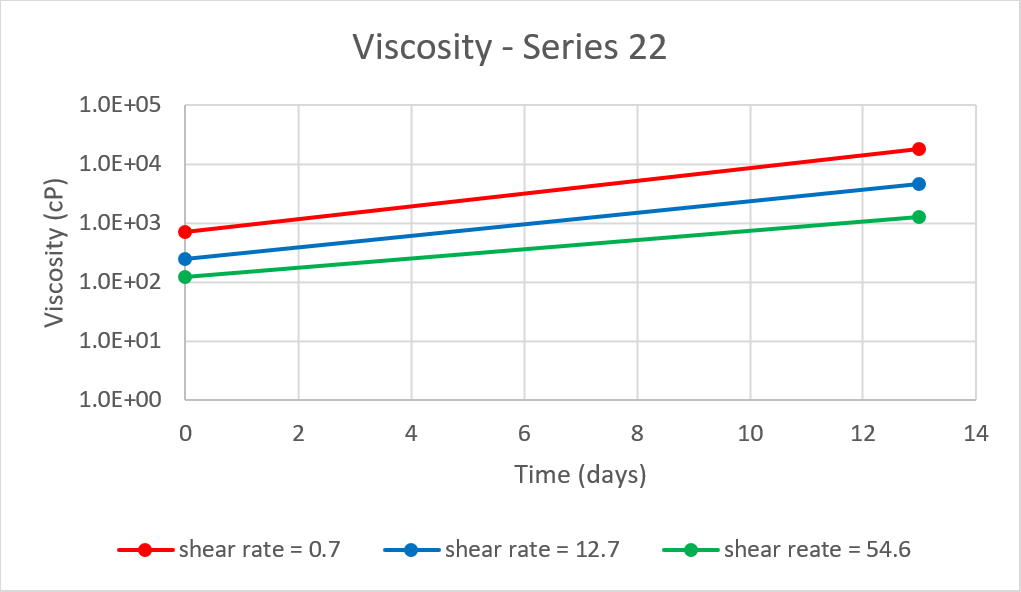
\includegraphics[width=\textwidth]{img/visc/22.png}
     \end{subfigure}
    }\\
    \makebox[\linewidth][c]{%
     \begin{subfigure}[b]{0.6\textwidth}
         \centering
         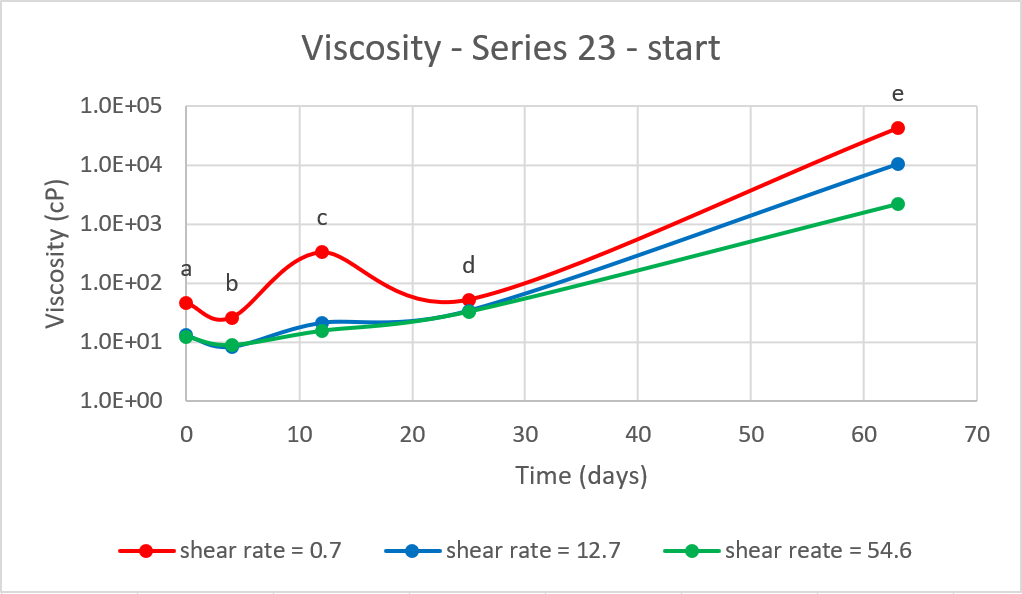
\includegraphics[width=\textwidth]{img/visc/23-1.PNG}
     \end{subfigure}
    %  \hfill
     \begin{subfigure}[b]{0.6\textwidth}
         \centering
         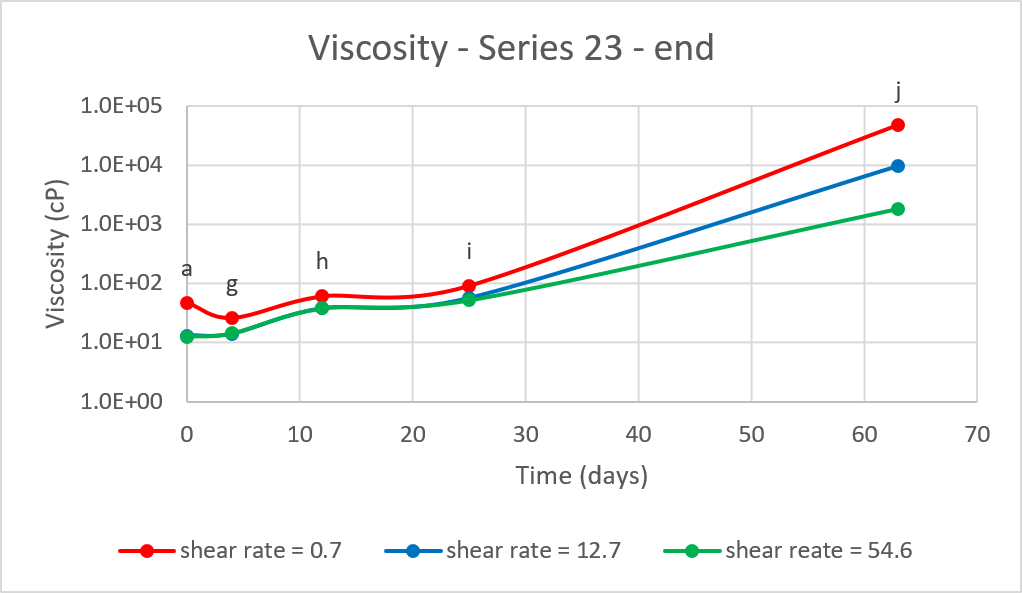
\includegraphics[width=\textwidth]{img/visc/23-2.png}
     \end{subfigure}
    }\\
        \caption{Viscosity vs. time, series 17 through 23}
        \label{fig:visc9-16}
\end{figure}


\begin{figure}
    \makebox[\linewidth][c]{%
     \begin{subfigure}[b]{0.6\textwidth}
         \centering
         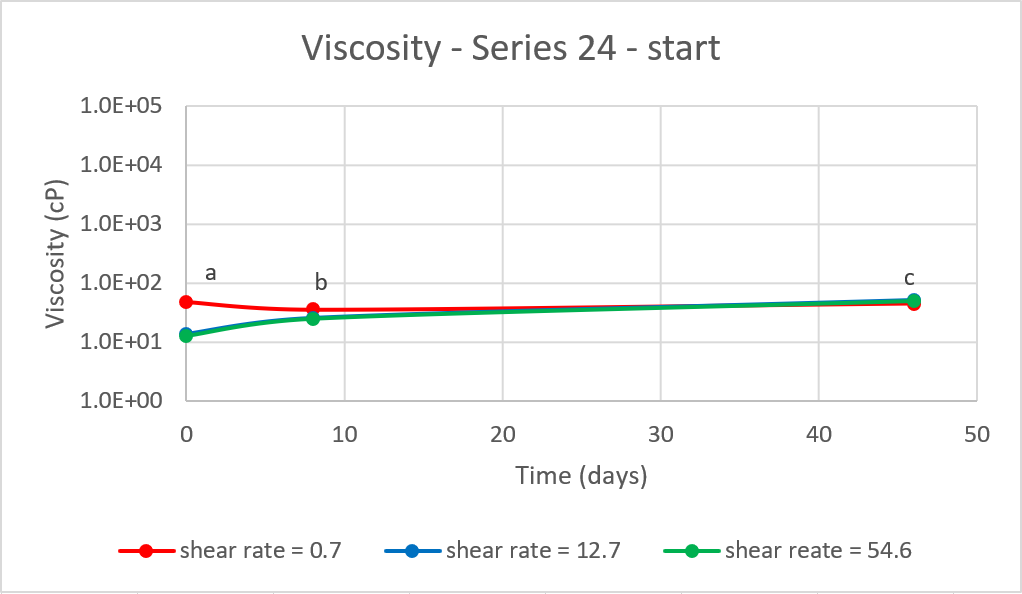
\includegraphics[width=\textwidth]{img/visc/24-1.png}
     \end{subfigure}
    %  \hfill
     \begin{subfigure}[b]{0.6\textwidth}
         \centering
         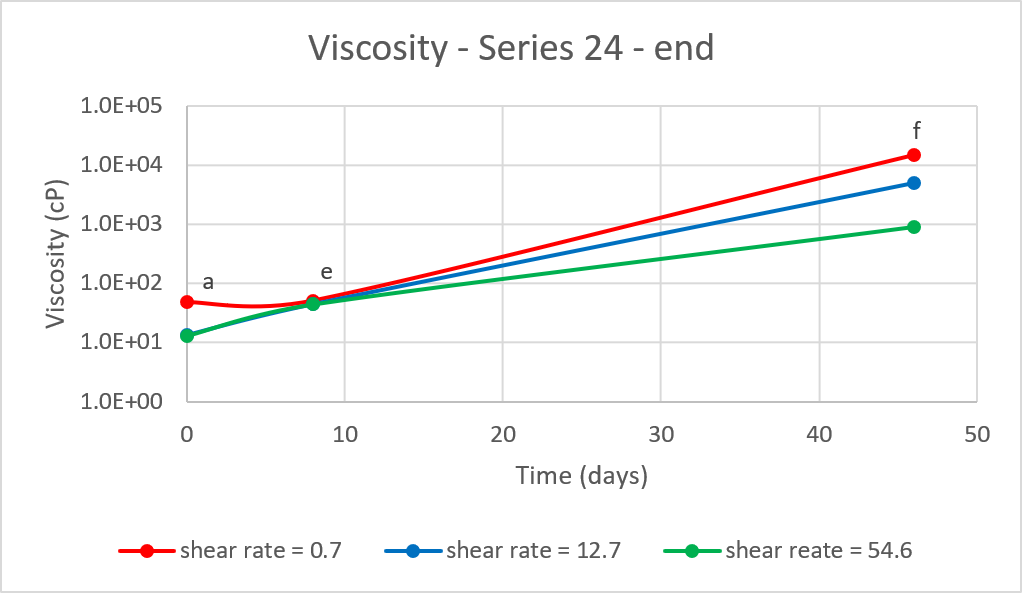
\includegraphics[width=\textwidth]{img/visc/24-2.png}
     \end{subfigure}
    }\\
    \makebox[\linewidth][c]{%
     \begin{subfigure}[b]{0.6\textwidth}
         \centering
         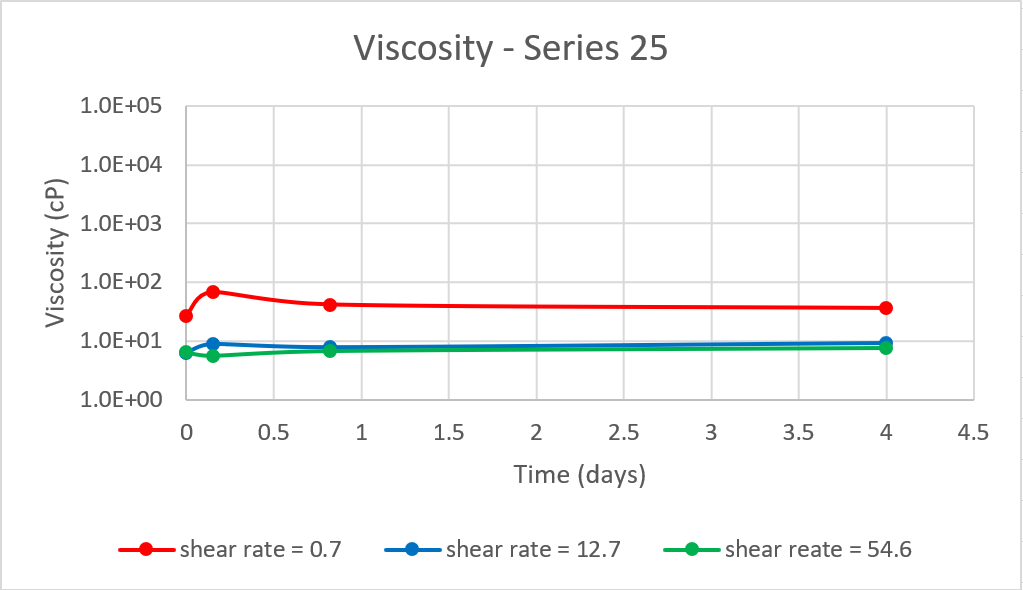
\includegraphics[width=\textwidth]{img/visc/25.png}
     \end{subfigure}
    %  \hfill
     \begin{subfigure}[b]{0.6\textwidth}
         \centering
         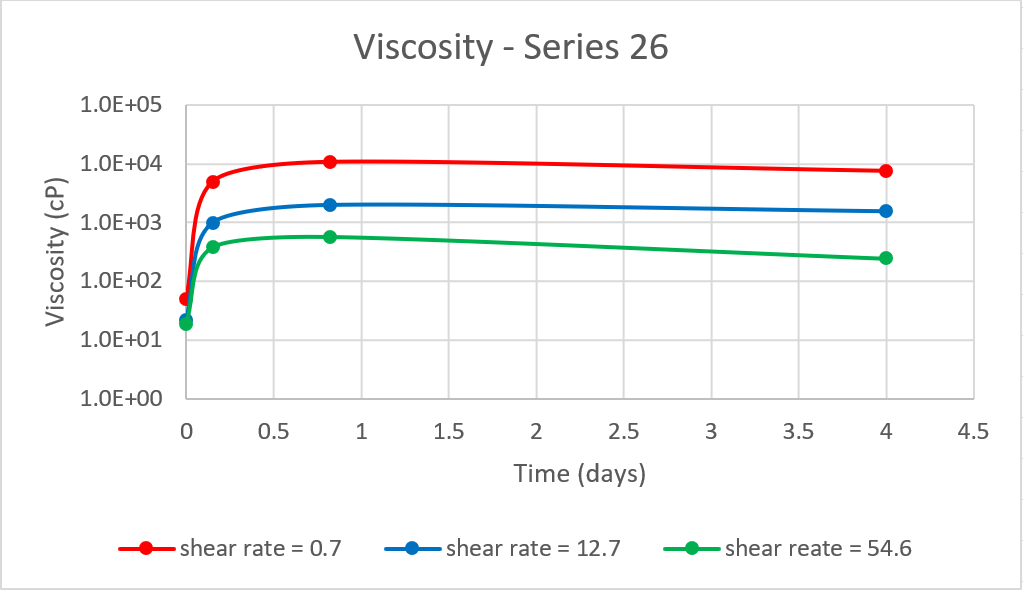
\includegraphics[width=\textwidth]{img/visc/26.png}
     \end{subfigure}
    }\\
    \makebox[\linewidth][c]{%
     \begin{subfigure}[b]{0.6\textwidth}
         \centering
         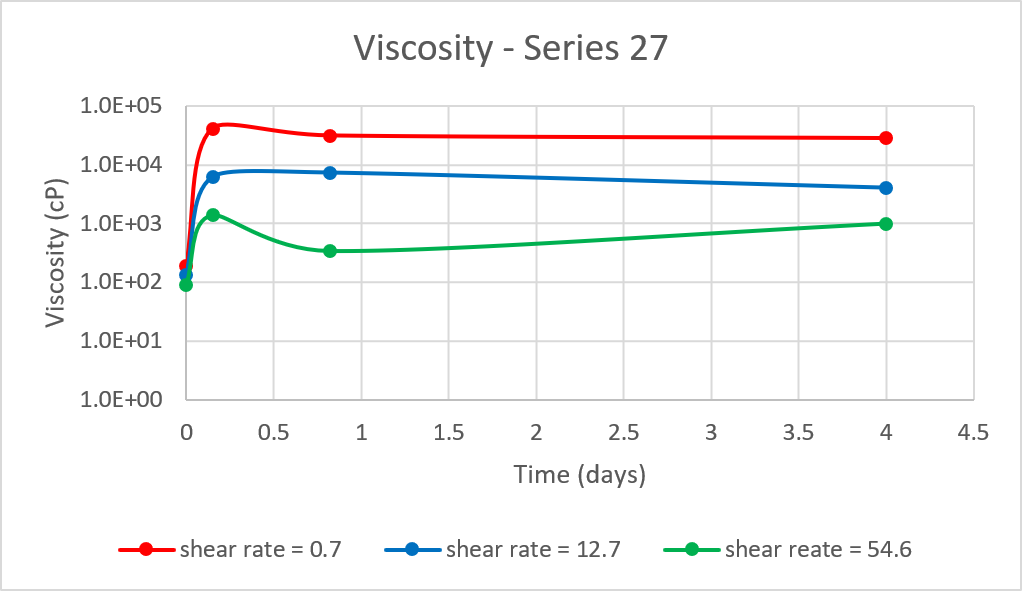
\includegraphics[width=\textwidth]{img/visc/27.png}
     \end{subfigure}
    %  \hfill
     \begin{subfigure}[b]{0.6\textwidth}
         \centering
         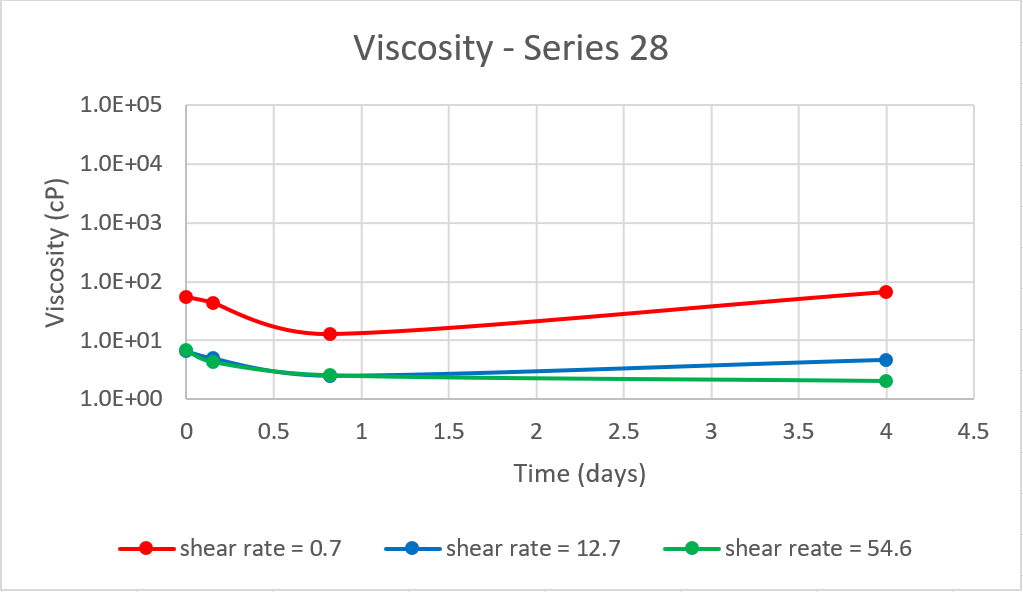
\includegraphics[width=\textwidth]{img/visc/28.png}
     \end{subfigure}
    }\\
    \makebox[\linewidth][c]{%
     \begin{subfigure}[b]{0.6\textwidth}
         \centering
         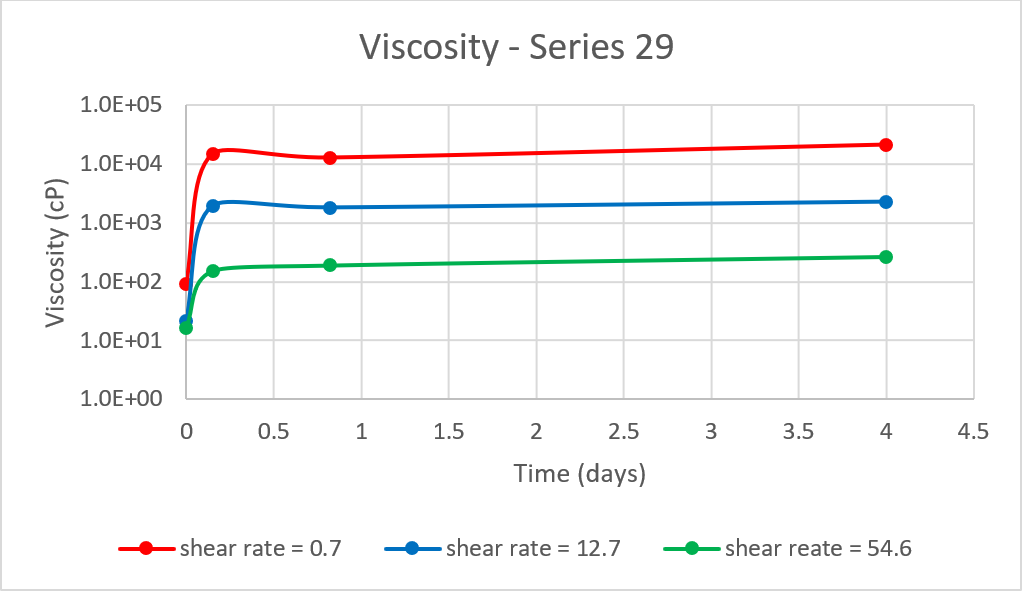
\includegraphics[width=\textwidth]{img/visc/29.png}
     \end{subfigure}
    %  \hfill
     \begin{subfigure}[b]{0.6\textwidth}
         \centering
         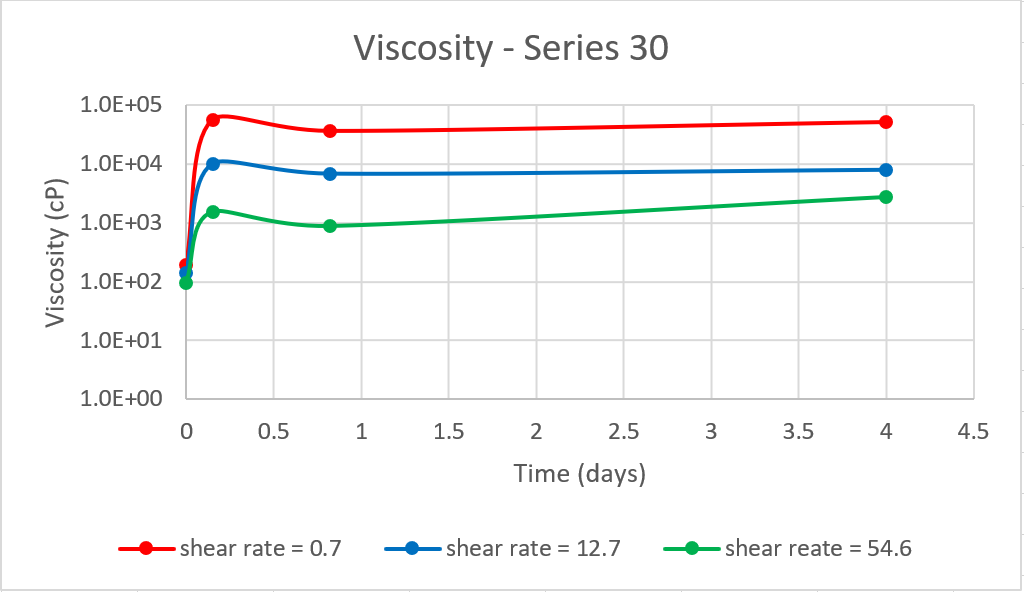
\includegraphics[width=\textwidth]{img/visc/30.png}
     \end{subfigure}
    }\\
        \caption{Viscosity vs. time, series 24 through 30}
        \label{fig:visc9-16}
\end{figure}


\begin{figure}
    \makebox[\linewidth][c]{%
     \begin{subfigure}[b]{0.6\textwidth}
         \centering
         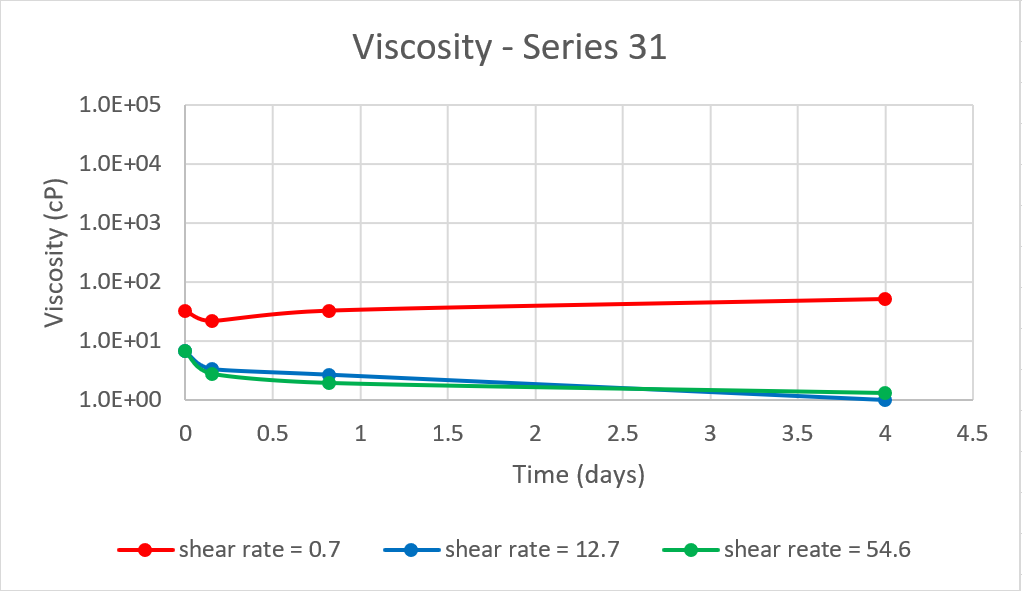
\includegraphics[width=\textwidth]{img/visc/31.png}
     \end{subfigure}
    %  \hfill
     \begin{subfigure}[b]{0.6\textwidth}
         \centering
         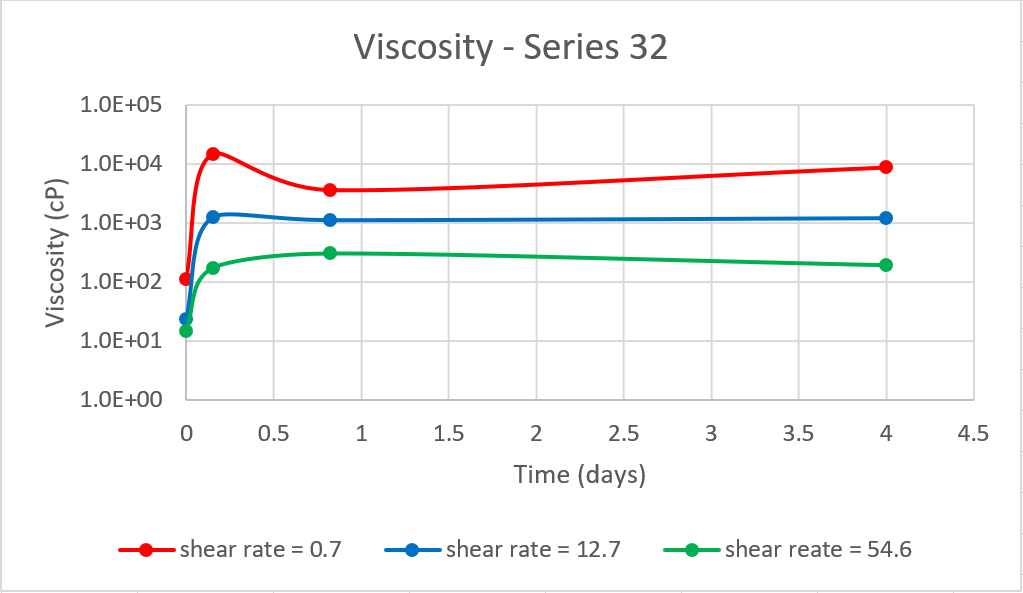
\includegraphics[width=\textwidth]{img/visc/32.png}
     \end{subfigure}
    }\\
    \makebox[\linewidth][c]{%
     \begin{subfigure}[b]{0.6\textwidth}
         \centering
         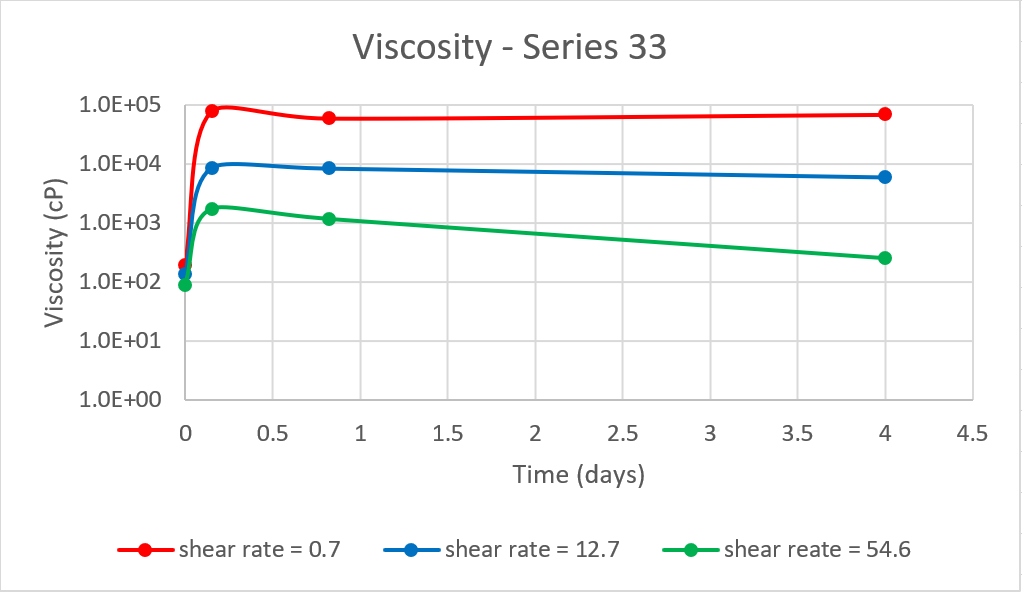
\includegraphics[width=\textwidth]{img/visc/33.png}
     \end{subfigure}
    %  \hfill
     \begin{subfigure}[b]{0.6\textwidth}
         \centering
         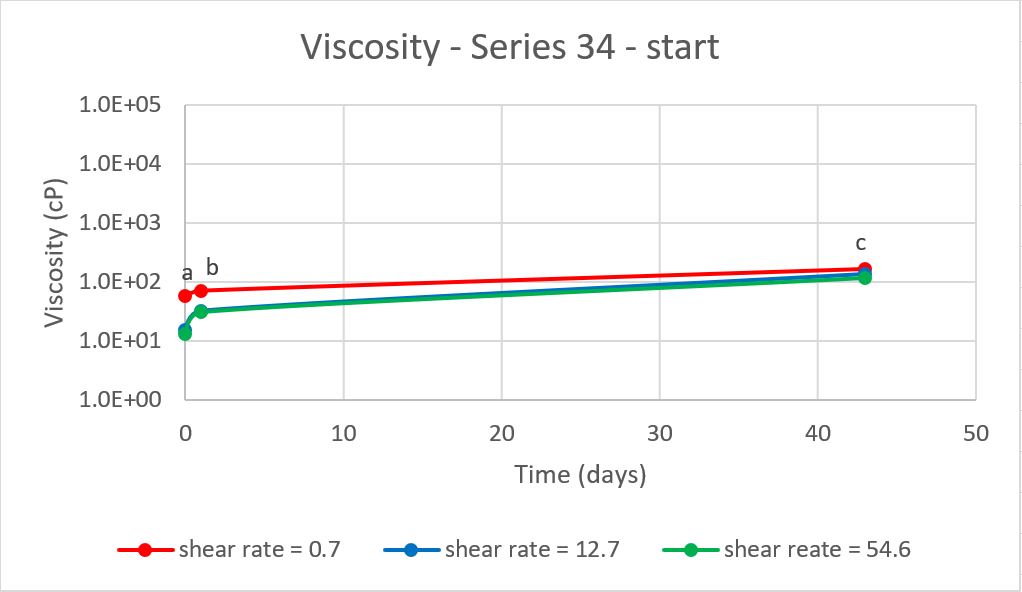
\includegraphics[width=\textwidth]{img/visc/34-1.png}
     \end{subfigure}
    }\\
    \makebox[\linewidth][c]{%
     \begin{subfigure}[b]{0.6\textwidth}
         \centering
         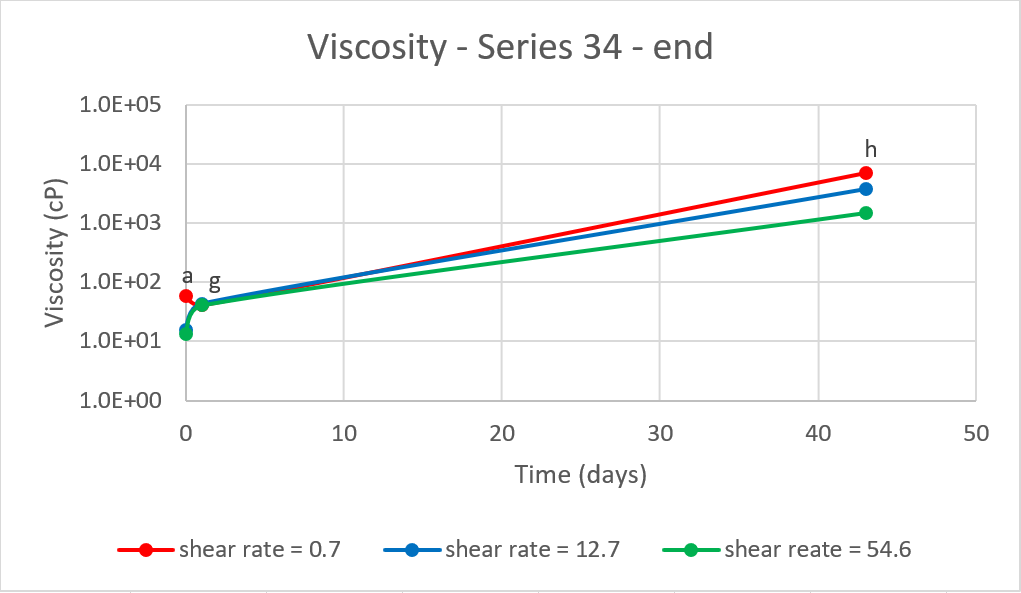
\includegraphics[width=\textwidth]{img/visc/34-2.png}
     \end{subfigure}
    %  \hfill
     \begin{subfigure}[b]{0.6\textwidth}
         \centering
         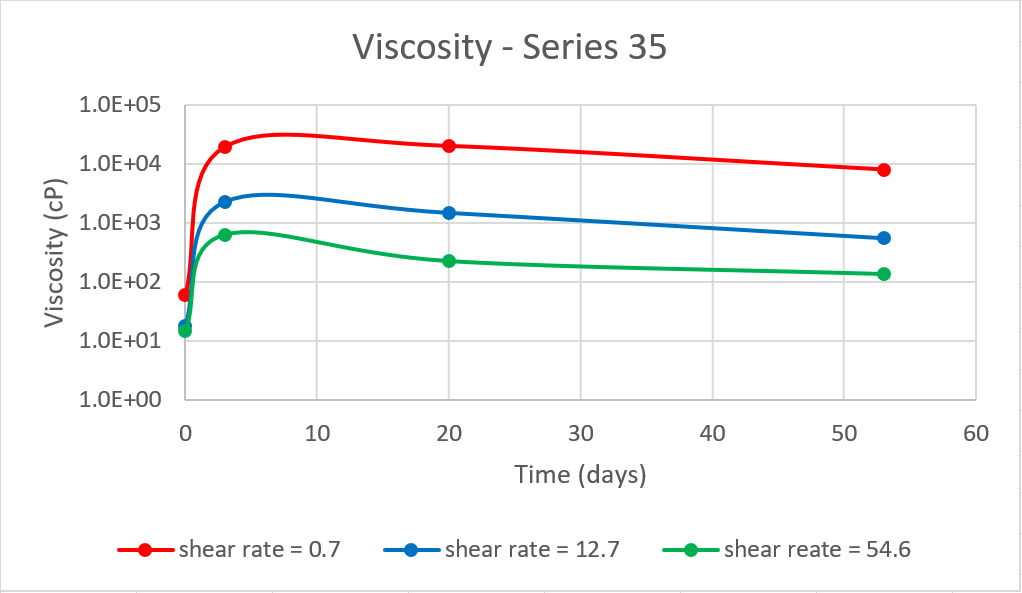
\includegraphics[width=\textwidth]{img/visc/35.png}
     \end{subfigure}
    }\\
    \makebox[\linewidth][c]{%
     \begin{subfigure}[b]{0.6\textwidth}
         \centering
         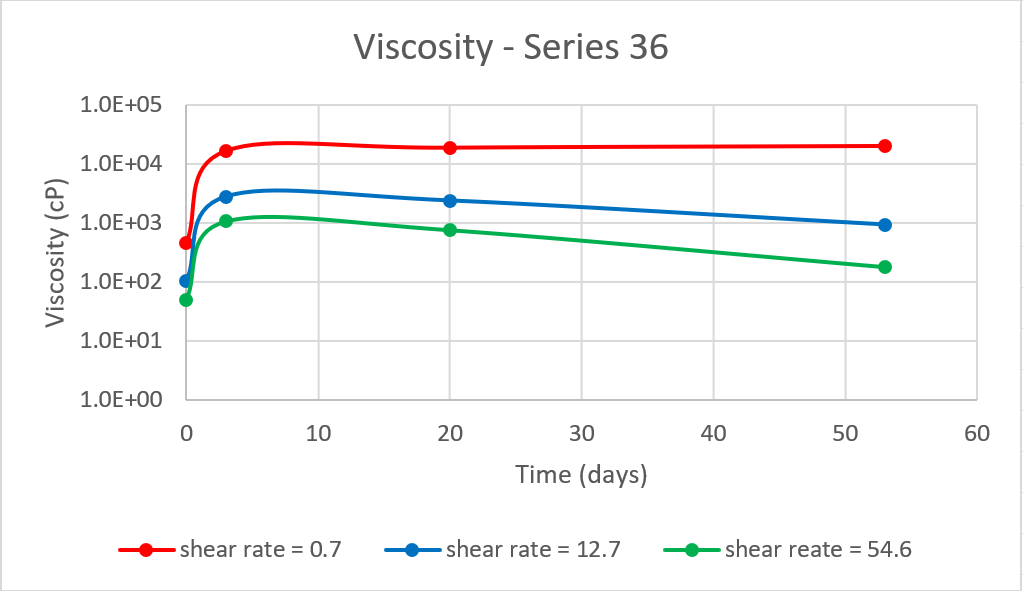
\includegraphics[width=\textwidth]{img/visc/36.png}
     \end{subfigure}
    %  \hfill
     \begin{subfigure}[b]{0.6\textwidth}
         \centering
         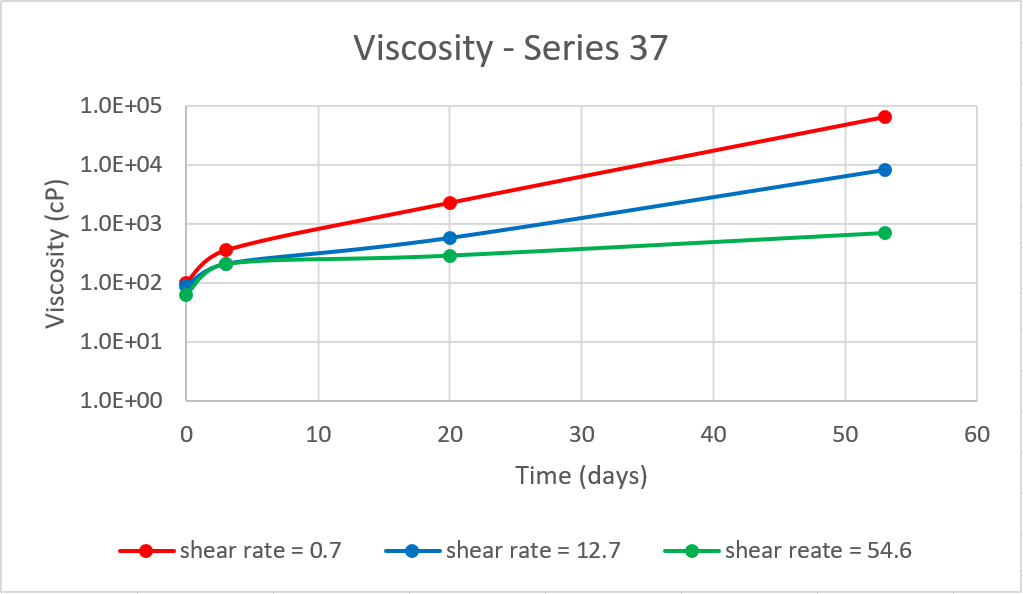
\includegraphics[width=\textwidth]{img/visc/37.png}
     \end{subfigure}
    }\\
        \caption{Viscosity vs. time, series 31 through 37}
        \label{fig:visc9-16}
\end{figure}


\begin{figure}
    \makebox[\linewidth][c]{%
     \begin{subfigure}[b]{0.6\textwidth}
         \centering
         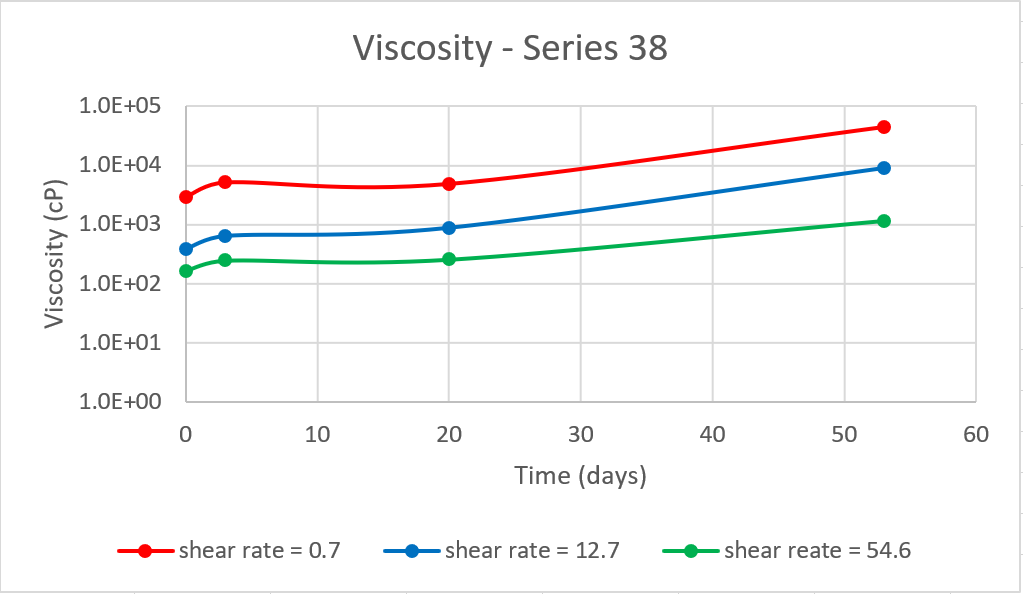
\includegraphics[width=\textwidth]{img/visc/38.png}
     \end{subfigure}
    %  \hfill
     \begin{subfigure}[b]{0.6\textwidth}
         \centering
         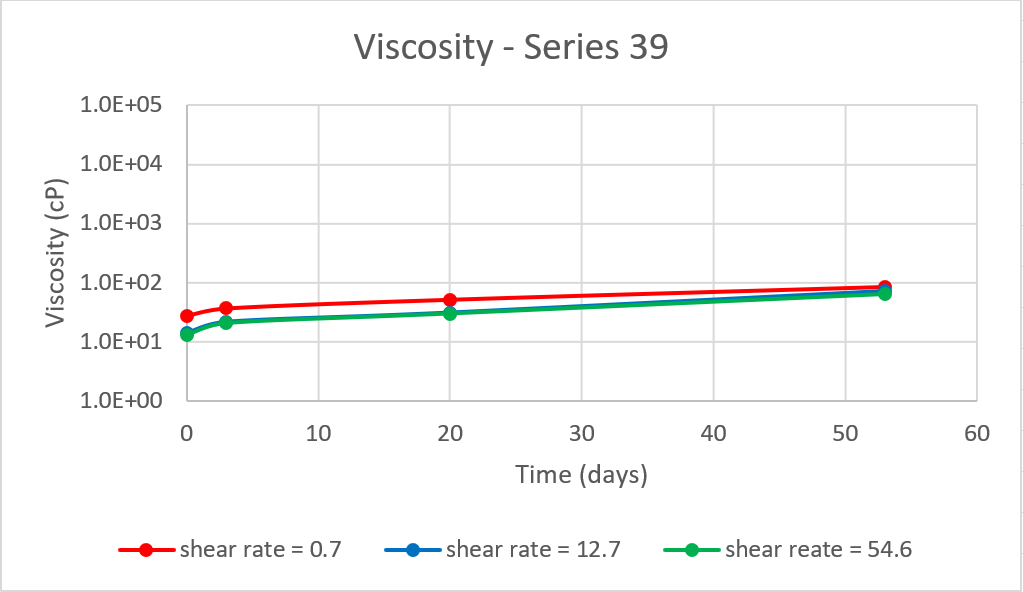
\includegraphics[width=\textwidth]{img/visc/39.png}
     \end{subfigure}
    }\\
    \makebox[\linewidth][c]{%
     \begin{subfigure}[b]{0.6\textwidth}
         \centering
         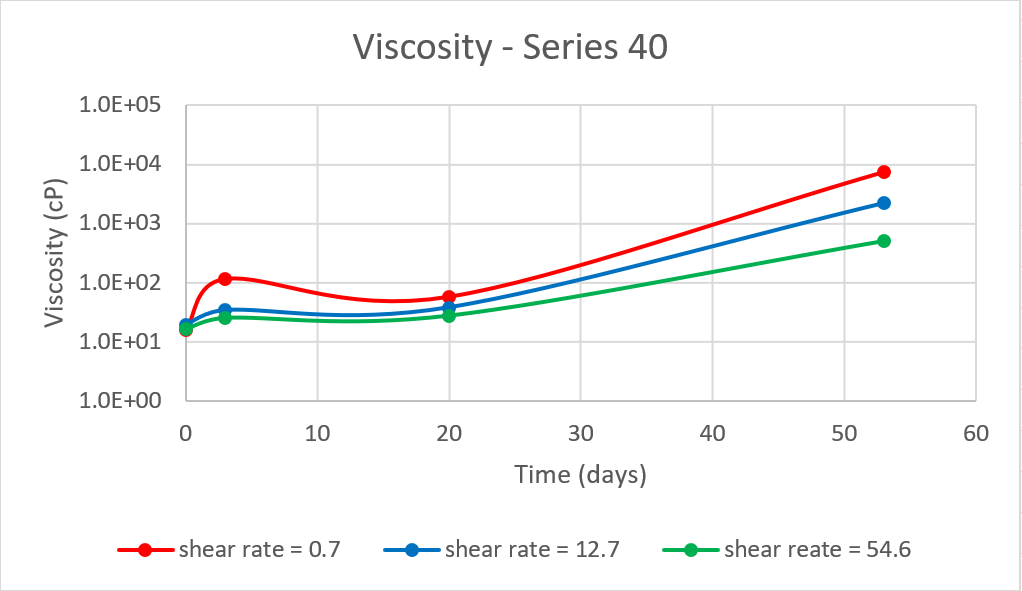
\includegraphics[width=\textwidth]{img/visc/40.png}
     \end{subfigure}
    %  \hfill
     \begin{subfigure}[b]{0.6\textwidth}
         \centering
         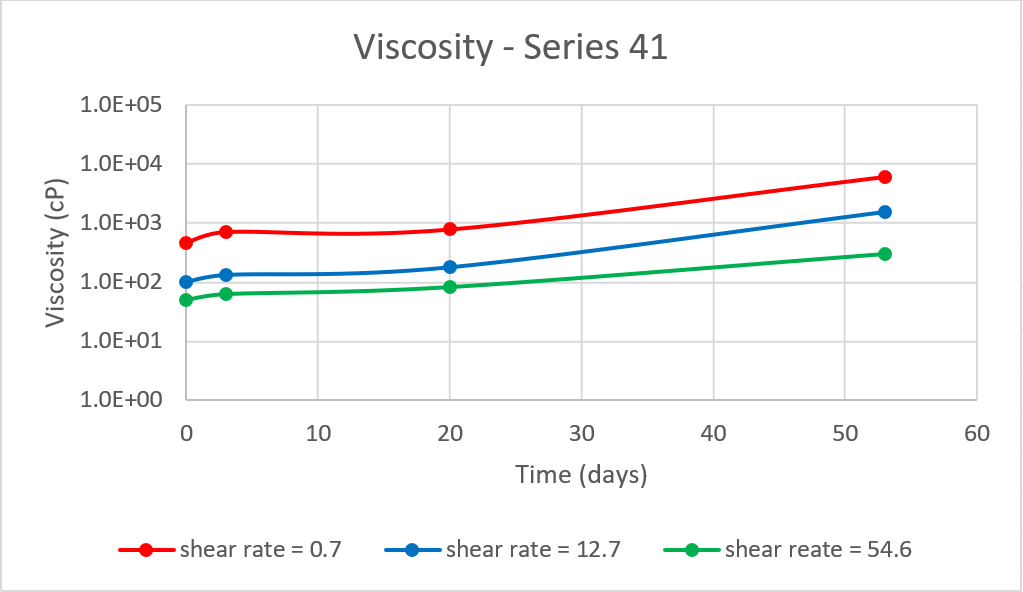
\includegraphics[width=\textwidth]{img/visc/41.png}
     \end{subfigure}
    }\\
    \makebox[\linewidth][c]{%
     \begin{subfigure}[b]{0.6\textwidth}
         \centering
         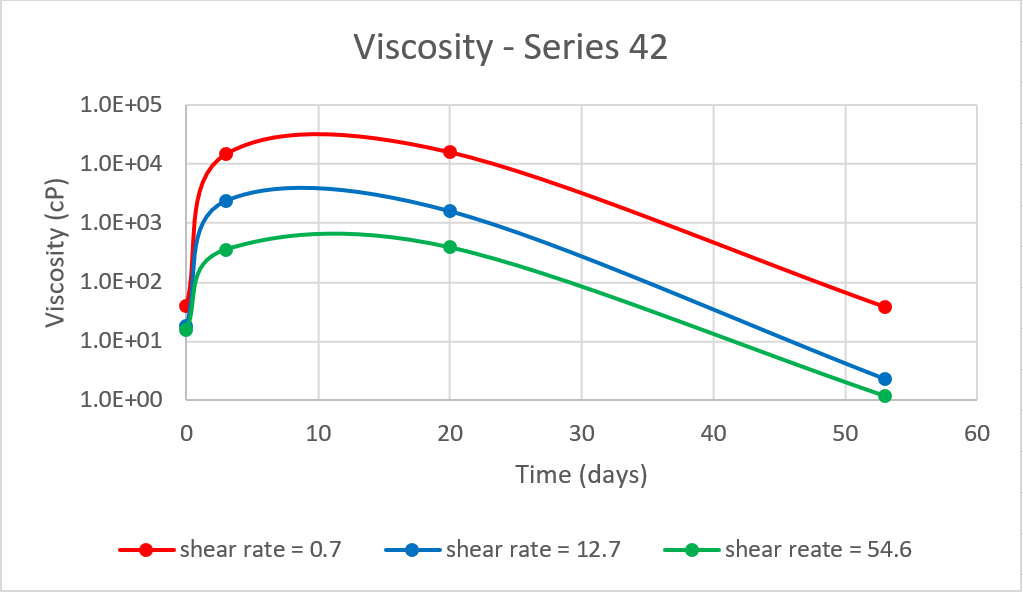
\includegraphics[width=\textwidth]{img/visc/42.png}
     \end{subfigure}
    %  \hfill
     \begin{subfigure}[b]{0.6\textwidth}
         \centering
         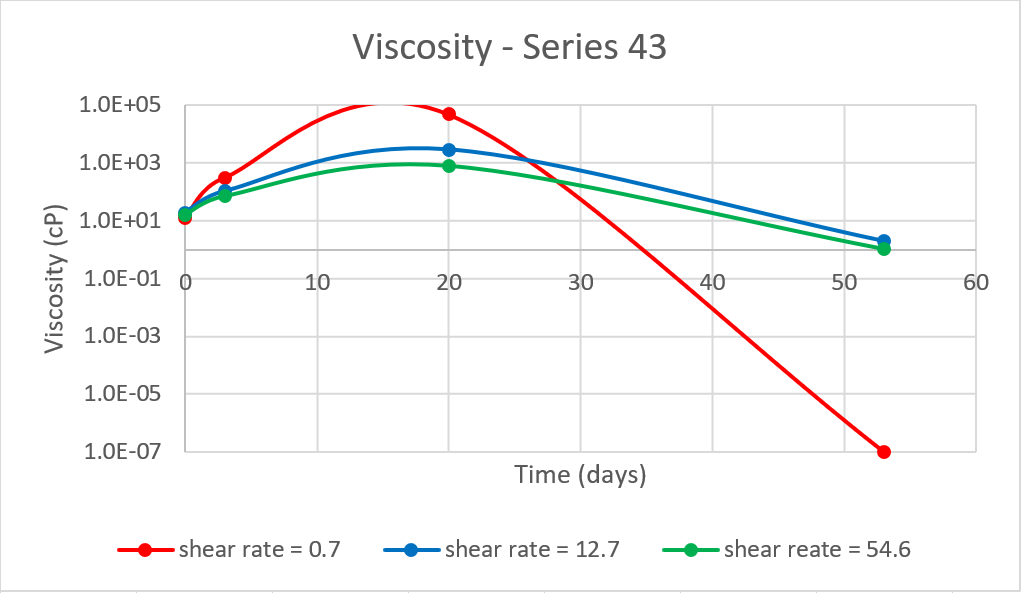
\includegraphics[width=\textwidth]{img/visc/43.png}
     \end{subfigure}
    }\\
    \makebox[\linewidth][c]{%
     \begin{subfigure}[b]{0.6\textwidth}
         \centering
         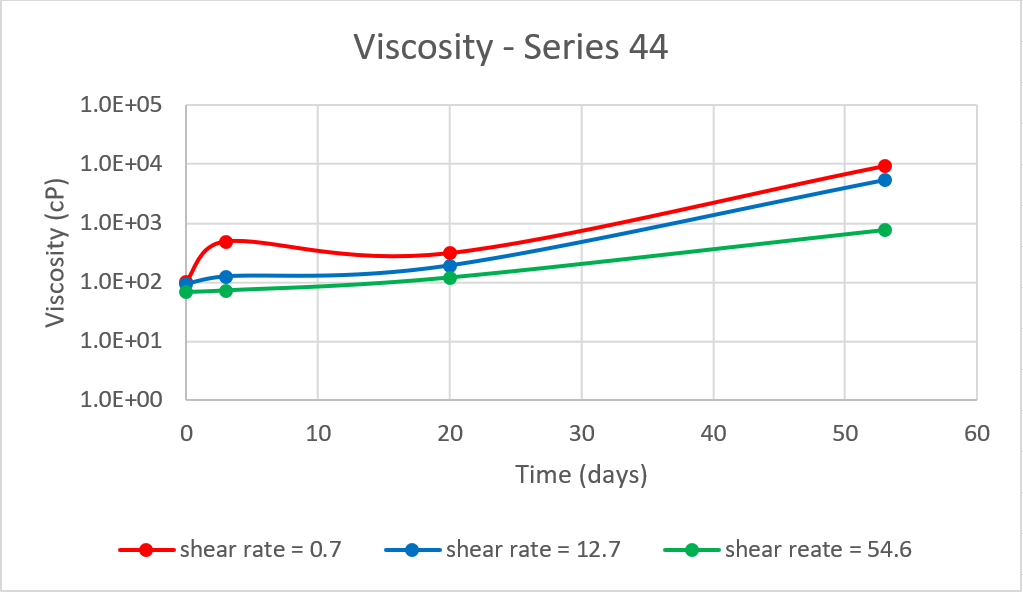
\includegraphics[width=\textwidth]{img/visc/44.png}
     \end{subfigure}
    %  \hfill
     \begin{subfigure}[b]{0.6\textwidth}
         \centering
         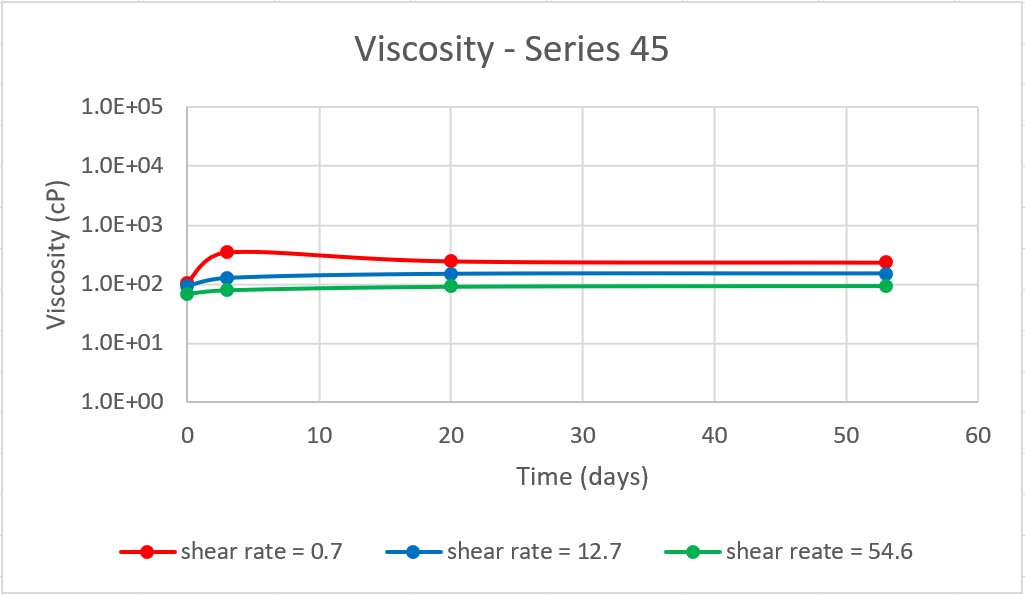
\includegraphics[width=\textwidth]{img/visc/45.png}
     \end{subfigure}
    }\\
        \caption{Viscosity vs. time, series 38 through 45}
        \label{fig:visc9-16}
\end{figure}


\begin{figure}
         \centering
         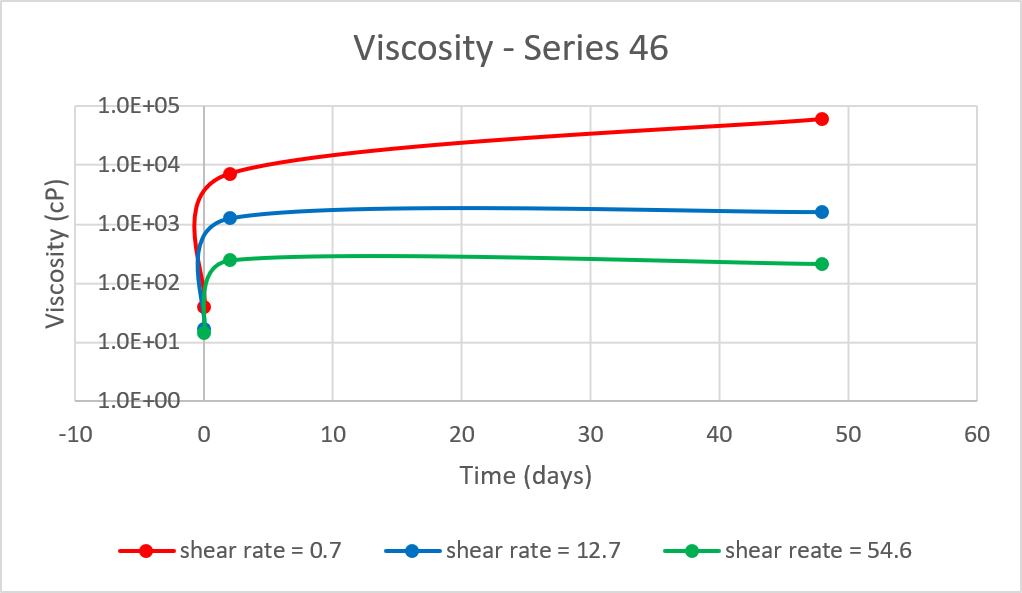
\includegraphics[width=.65\textwidth]{img/visc/46.png}
         \caption{Viscosity vs. time, series 46}
         \label{fig:visc46}
\end{figure}

\chapter{Simulator Input \label{chap:simInput}}
\lstset{language=C}

The mathematical and numerical model has been implemented in an approximately 3000 lines long c-code. The simulator is relatively fast and seems robust with regards to convergence. The input for a simulation case is file based with a certain fixed format. 

Input file
In the input file example below, all additional explanatory text (comments) are included and the text is bracketed with /*    */. Remove the text before the file can be used as input or control file for the simulator. Actual keywords and parameters are in bold.
 

\textbf{1D NANO-SIMULATOR.}
The following is a specification of input format for the 1D nano-simulator.
The input format is fixed, only white space between entries can have an arbitrary number of blanks, end of lines, or tabs (complying to the fscanf routine in c). The order of the keywords must be as in the example below. Keywords are not read and interpreted.
Keywords (or some string) and units (or some string) must be explicitly included in the text as given below, as the program expects strings just as in the example below.
Note that for a real input file no comments can be included, \textit{i.e.,} everything bracketed with /*  */ must be removed in this example file before the executive nano-simulator can read it properly. 
Not all keywords are commented below. Inputs that are self-explanatory are uncommented.
 

\begin{lstlisting}

/******************************************
`Testcase1' is the title of the simulation 
*******************************************/
Title Testcase1

/***************************************
nx is number of grid blocks, CrossArea is the 
cross sectional area of the model.
****************************************/
nx 100
Lenght 100.0 cm
CrossArea 25.0 cm^2

/*****************************************************
Initial water saturation can either be constant 
(as here) or have nx entries. If the first number
after keyword `InitialWaterSaturation' is 0, then
a single constant value for initial water saturation
is expected. Any other value for this first parameter, 
the program expects nx real numbers to be read. 
******************************************************/  
InitialWaterSaturation 0 0.7
Permeability 1000.0 mD
Porosity 0.3

/*****************************************************
When nano particles and/or polymer is present, there 
may be inaccessible pore space for these particles
in solution. Therefore, we have defined two additional 
porosities.
******************************************************/
PorosityNano 0.25
PorosityPolymer 0.2

/*****************************************************
Adsorption isotherms are specified by mass adsorbed 
per mass rock in the tables below. The rock 
density is therefore required 
******************************************************/
RockDens 2.5 g/cm^3

/*****************************************************
Assuming Corey type of relative permeability. No 
capillary forces or gravity.
******************************************************/
IrreducibleWaterSat 0.3
ResidualOilSat 0.2
WaterRelPermEndValue 0.6
OilRelPermEndValue 0.9
CoreyExponentWater 2.0
CoreyExponentOil 3.0

/*****************************************************
Boundary conditions are given by injection rate 
(Neuman type). To calculate the pressures during the
simulation a reference pressure at the end of the model 
is needed.
*****************************************************/
BackPressure 1.0 bar

/****************************************************
Oil viscosity is constant. Absolute permeability can 
be reduced by adsorbed polymer, affecting the oil 
rate. See keyword `AdsorptionPolymer'.
*****************************************************/
OilVisc 0.5 cP

/******************
Water mass density.
******************/
WatDens 1.0 g/cm^3

/****************************************************
The first number after the keyword `WaterViscPolymer'
gives the number of lines in the table. The table 
defines the effect of polymer on water viscosity when 
no crosslinking has occurred, where the second column
is a multiplicator giving the relative change in water 
viscosity as a function of polymer concentration in the water. 
*****************************************************/
WaterViscPolymer 5
g/g    
0.0	1.0  
0.001  	2.0
0.003  	6.0
0.007  	10.0
0.01   	12.0

/*****************************
Water viscosity for pure brine
******************************/
WaterViscosity 0.5 cP

/******************************************************
Maximal possible water viscosity (maximal gel strength) 
*******************************************************/
MaxGelWaterViscosity 1000.0 cP

/*************************************************
Reference rate for calculation of shear thinning 
of water viscosity
**************************************************/ 
ReferenceRate 4.0 cm^3/hr

/****************************************************
Reduction in water viscosity due to shear thinning is
a tabulated function of polymer concentration and 
relative rate (relative to `Reference rate'). Integer
after `PolymerConcentration' is number of entries of 
the first variable, and integer after `RateRatio' is
number of entries of second variable.
*****************************************************/
PolymerConcentration 4
g/g
0.0    
0.001  
0.003  
0.007  
0.01   

RateRatio 4
0.5
0.8
1.0
1.5

/****************************************************
Factor multiplied with water viscosity due to shear 
thinning. First group of values for first value of polymer
concentration and increasing RateRatio. Then next for next
value of polymer concentration.
******************************************************/
ShearFactor
1.0	1.0	1.0	1.0	
0.9	0.88	0.86	0.83
0.88	0.83	0.8	0.77
0.86	0.8	0.75	0.7

/******************************************************
Tables of nano particle concentration and polymer 
concentration for the two-variable function h involved 
in calculation of water viscosity. Again, the number after
`NanoConcentration' and `Polymerconcentration' define the
number of entries in each table.
*******************************************************/ 
NanoConcentration 5
g/g  
0.0 
0.0001
0.0002
0.0004
0.0006

Polymerconcentration 5
g/g
0.0    
0.001  
0.003  
0.007  
0.01   

/*****************************************************
Values for the two-variable function h. The nano 
concentrations are in the outer loop and here the first
5 values correspond to the first nanoconcentration, with
increasing polymer concentrations. The next 5 values are
for the second nano concentration, with increasing 
polymer concentration etc.
******************************************************/
hFunction
0.0	0.0  	0.0  	0.0  	0.0
0.0  	0.01	0.03	0.05	0.1
0.0	0.04	0.1	0.2	0.4
0.0	0.1	0.3	0.5	0.7
0.0	0.15	0.45	0.75	1.0

/*****************************************************
The first column is times, while the second column is 
values for the age function. This function describes 
the strength of the gel as a function of age of the 
nano particles. The number after the keyword 
is number of entries in the table. 
******************************************************/
AgeFunction 10 
hr 
10.0 	0.0
11.0 	0.01
12.0 	0.03
13.0 	0.06
13.5 	0.1
14.0 	0.2
14.25 	0.35
14.5  	0.55
14.75 	0.75
15.0  	1.0

/*****************************************************
Adsorption isotherms for nanoparticles. The first 
number after the keyword is the number of lines in the
table. The second number is zero if there is no 
desorption of nanoparticles. Any other value means
that desorption takes place if nanoparticle concentration
in water decreases.   
******************************************************/
AdsorptionNano 5  0
g/g     	g/g_rock
0.0     	0.0
0.0001  	0.00001
0.0002  	0.00002
0.0004  	0.00004
0.0006  	0.00006

/*****************************************************
Adsorption isotherms for polymer. The first number after
the keyword is the number of lines in the table.
The second number is zero if there is no resorption of 
polymer particles. The third column in the table gives 
the reduction factor for absolute permeability as a 
function of adsorbed polymer concentration.
******************************************************/ 
AdsorptionPolymer 5  0
g/g    	g/g_rock
0.0    	0.0      	1.0
0.001  	0.0001   	0.7
0.003  	0.0003   	0.5
0.007  	0.0007   	0.3
0.01   	0.001    	0.2

/*****************************************************
`PrintOutFreq' is number of time steps between each 
output to files of position dependent data. 
`root' is the name of the input file. Dynamic data 
written to separate files are:

pressure root.PR
water saturation root.SAT
nanoparticle concentration root.NAN 
polymer concentration root.POL
adsorbed nanoparticle concentration root.ADNAN 
adsorbed polymer concentration root.ADPOL
water viscosity root.WATVISC
absolute permeability root.PERM
age profile for nanoparticles in solution root.AGENANSOL
age profile for absorbed nanoparticles root.AGENANADS

Scalar values (single values at each time step) are 
written to root.SCALAR at each time step. These include
injection and production rates for water, oil, nanoparticles
and polymers. In addition, numerical data such as time step, 
number of Newton iterations, number of linear iterations, 
time step cut backs, and position and magnitude of maximal
water viscosity change. These data are written to root.NUM 
***********************************************************/
PrintOutFreq 5

/****************************************************
Gives minimal time between print outs. Overrides 
previous keyword if time steps become very small.
*****************************************************/
MinTimeBetweenPrintOut 0.1 hr

/****************************************************
 Factor for cutting time step in case of 
 non-convergence or violation of other criteria.
*****************************************************/
TimeStepCutBackFactor 0.3

/******************************************
Increase factor for next time step length.
*******************************************/
TimeStepIncreaseFactor 1.1

/***********************
Minimal time step length.
************************/
MinTimeStep 0.005 hr

/***********************
Maxmal time step lenght.
************************/
MaxTimeStep 0.5 hr

/*********************************************
 Maximum iterations for linear equation solver.
**********************************************/
MaxLinItr 10

/*************************
Maximum Newton iterations.
**************************/
MaxNewtonItr 7

/*****************************
Tolerance for linear iteration
******************************/
ToleranceLinear 1.0e-6

/*****************************
Tolerance for Newton iteration
******************************/
ToleranceNewton 1.0e-6

/***********************************
Relaxation parameter in SOR routine 
for solving linear equations
************************************/
Relaxation 1.5

/**************************************************
Maximum change in water viscosity in one time step.
**************************************************/
MaxDeltaWatVisc 5.0 cP

/*************************************************
Define the first time step lenght by giving pore 
volume water injected at first time step.
**************************************************/
InitPVInj 0.003 PV

/****************************************************
Reference values for scaling nanoparticle and polymer
conservation equation in calculation of norm of
residual in Newton iteration 
*****************************************************/
ReferenceNanoCon 0.0006 g/g
ReferencePolyCon 0.01 g/g

/****************************************************
Last comes the schedule file specifying the boundary 
conditions which are, in general, time dependent. The
number after `Times' is the number of tables specifying 
boundary conditions. Each table has 4 lines:

1. The time interval for the boundary conditions.
2. Solution (water) injection rate.
3. Concentration of nano particles injected in solution.
4. Concentration of polymers injected in solution.
*****************************************************/
Times 4

Time 0.0  3.0 hr
Rate 2.0 cm^3/hr
NanoConcentration 0.0005 g/g
PolymerConcentration 0.008 g/g

Time 3.0  15.0 hr
Rate 2.0 cm^3/hr
NanoConcentration 0.000 g/g
PolymerConcentration 0.00 g/g

Time 15.0  17.0 hr
Rate 2.0 cm^3/hr
NanoConcentration 0.0005 g/g
PolymerConcentration 0.008 g/g

Time 17.0  30.0 hr
Rate 2.0 cm^3/hr
NanoConcentration 0.0 g/g
PolymerConcentration 0.0 g/g

\end{lstlisting}

\end{appendices}
\clearpage